\chapter{Obdelava slik}\label{sec:ObdelavaSlik}
%
Pri obdelavi signalov in v teoriji filtrov je Fourierova transformacija še vedno zelo močno orodje, ki se ga lahko uporablja za odstranjevanje šuma, pohitritev računanja konvolucije dveh matrik, izboljšavo kakovosti signala \ldots

V prvem razdelku tega poglavja si bomo zato najprej pogledali teoretično ozadje za Fourierovo transformacijo in njeno izboljšano različico (hitro Fourierovo transformacijo). V našem delu se bomo ukvarjali le z obdelavo slik, zato bomo v pretežni meri vso teorijo in izpeljane postopke aplicirali na slike, čeprav bo vse skupaj v prilagojenih različicah veljalo tudi za ostale vrste signalov.

V drugem razdelku bomo nato spoznali nekaj osnovnih pojmov in postopkov iz teorije filtrov. Našteli bomo osnovne vrste transformacij slike, se naučili postopkov za njihov izračun in nato predstavili osnovne filtrirne postopke (zaznava robov na sliki, zameglitev slike, glajenje robov na sliki \ldots), ki jih bomo uporabljali v algoritmih za likovno upodabljanje slik.

V tretjem razdelku se bomo posvetili barvnim prostorom RGB, CMY, HSV in YUV. Spoznali bomo tudi Kubelka-Monk barvni model, ki ga bomo uporabili v algoritmu za likovno upodabljanje slik z voščenkami.

% Ta odstavek ni nujno resničen.
Pri obdelavi slik je postopek odstranjevanja šuma zelo pomemben, zato si bomo v zadnjem razdelku tega poglavja pogledali različne algoritme za odstranjevanje šuma. Gaussovo filtriranje je postopek za odstranjevanje šuma, ki je sicer hiter, vendar pa nam večkrat vrne nezadovljive rezultate. Na drugi strani pa bomo spoznali še nelokalno odstranjevanje šuma s slike, ki da zelo dobre rezultate, vendar pa ima kljub temu, da lahko nekatere izračune v algoritmu pohitrimo, še vedno kvadratno časovno zahtevnost. V algoritmih za likovno upodabljanje slik bomo odvisno od naših trenutnih prioritet (hitrost ali kakovost) izbrali ustrezni postopek za odstranjevanje šuma.
%
%%%  Razdelek Fourierova transformacija.
\section{Fourierova transformacija}\label{sec:FourierT}
%
V tem razdelku bomo predstavili teorijo, ki nas bo vodila do algoritma za izračun dvodimenzionalne hitre (diskretne) Fourierove transformacije. Teorijo bomo povzeli po~\cite[2.~poglavje]{Frazier:AnIntro} in njene rezultate skupaj z dokazi zapisali za dvodimenzionalno različico ter jih opremili z lastnimi primeri.
%% Fourierova baza.
\subsection{Fourierova baza}
%
Najprej bomo definirali $N$-dimenzionalni vektorski prostor $\l^2(\Z_N)$ nad kompleksnimi šte\-vi\-li:
$$\l^2(\Z_N) \coloneqq \set{z = (z(0), z(1), \ldots, z(N-1)) \mid z(j) \in \C, 0 \leq j \leq N-1}.$$
Prostor bomo opremili s standardno evklidsko bazo $E = \set{e_0, e_1, \ldots, e_{N-1}}$, kjer za bazni element $e_j$ velja: $e_j(n) = 1$ za $j=n$ in $e_j(n) = 0$ sicer. V nadaljevanju bomo definirali prostor $l^2(\Z_{N_1} \times \Z_{N_2})$, ga opremili s standardno bazo in nato spoznali Fourierovo bazo.
%
\begin{definicija}
  Za naravni števili $N_1$ in $N_2$ definiramo
  $$\l^2(\Z_{N_1} \times \Z_{N_2}) \coloneqq \set{\fun{z}{\Z_{N_1} \times \Z_{N_2}}{\C}}\;.$$
\end{definicija}
%
Elemente $z \in \l^2(\Z_{N_1} \times \Z_{N_2})$ lahko zapišemo tudi z matriko
%
\begin{equation*}
  z =
    \begin{bmatrix}
      z(0, 0) & z(0, 1) & \hdots & z(0, N_2-1)\\
      \vdots & \vdots & \ddots & \vdots\\
      z(N_1-1, 0) & z(N_1-1, 1) & \hdots & z(N_1-1, N_2-1)
    \end{bmatrix}\;,
\end{equation*}
%
kjer so za $0 \leq n_1 \leq N_1-1, 0 \leq n_2 \leq N_2-1$ vrednosti $z(n_1, n_2) \in \C$.

Z običajnim seštevanjem in množenjem s skalarjem po komponentah postane množica $\l^2(Z_{N_1} \times Z_{N_2})$ vektorski prostor nad $\C$. Za elementa $z, w \in \l^2(Z_{N_1} \times Z_{N_2})$ definiramo kompleksni skalarni produkt
%
\begin{equation}\label{eq:defSP}
  \langle z, w\rangle \coloneqq \sum_{n_1 = 0}^{N_1 - 1} \sum_{n_2 = 0}^{N_2 - 1} z(n_1, n_2)\overline{w(n_1, n_2)} \;.
\end{equation}
%
\begin{trditev}
Prostor $\l^2(\Z_{N_1} \times \Z_{N_2})$ je $N_1 N_2$-dimenzionalen.
\end{trditev}
%
\begin{dokaz}
Dimenzija prostora je enaka razsežnosti njegove baze. Definiramo množico
$$E = \set{e_{i,j} \mid 0 \leq i \leq N_1-1, 0 \leq j \leq N_2-1},$$
kjer je $e_{i,j}(n_1, n_2) = 1$ za $(i, j) = (n_1, n_2)$ in $e_{i,j}(n_1, n_2) = 0$ sicer. Zanjo enostavno preverimo, da je linearno neodvisna in razpenja celoten prostor $\l^2(\Z_{N_1} \times \Z_{N_2})$, torej je $N_1N_2$-razsežna baza prostora $\l^2(\Z_{N_1} \times \Z_{N_2})$.
\end{dokaz}
%
\begin{izrek}
Naj bosta $\set{B_0, B_1, \ldots, B_{N_1 - 1}}$ in $\set{C_0, C_1, \ldots, C_{N_1 - 1}}$ ortonormirani bazi za $\l^2(\Z_{N_1})$ in $\l^2(\Z_{N_2})$. Za $0 \leq m_1 \leq N_1 - 1$ in $0 \leq m_2 \leq N_2 - 1$ naj bo
$$D_{m_1, m_2}(n_1, n_2) \coloneqq B_{m_1}(n_1)C_{m_2}(n_2) \;.$$
Tedaj je $\set{D_{m_1, m_2}}_{0 \leq m_1 \leq N_1 - 1, 0 \leq m_2 \leq N_2 - 1}$ ortonormirana baza prostora $\l^2(\Z_{N_1} \times \Z_{N_2})$.
\end{izrek}
%
\begin{dokaz}
Najprej preverimo, da velja enakost $\langle D_{m_1, m_2}, D_{k_1, k_2}\rangle = \langle B_{m_1}, B_{k_1} \rangle \langle C_{m_2}, C_{k_2}\rangle$. Z uporabo definicije skalarnega produkta \eqref{eq:defSP} in s preureditvijo členov v dvojni vsoti dobimo:
%
\begin{align*}
\langle D_{m_1, m_2}, D_{k_1, k_2}\rangle & = \sum_{n_1 = 0}^{N_1 - 1} \sum_{n_2 = 0}^{N_2 - 1} D_{m_1, m_2}(n_1, n_2)\overline{D_{k_1, k_2}(n_1, n_2)} \\
& = \sum_{n_1 = 0}^{N_1 - 1} \sum_{n_2 = 0}^{N_2 - 1} B_{m_1}(n_1)C_{m_2}(n_2) \overline{B_{k_1}(n_1)C_{k_2}(n_2)} \\
& = \sum_{n_1 = 0}^{N_1 - 1} \sum_{n_2 = 0}^{N_2 - 1} B_{m_1}(n_1)\overline{B_{k_1}(n_1)}C_{m_2}(n_2) \overline{C_{k_2}(n_2)} \\
& = \sum_{n_1 = 0}^{N_1 - 1} B_{m_1}(n_1)\overline{B_{k_1}(n_1)} \sum_{n_2 = 0}^{N_2 - 1} C_{m_2}(n_2) \overline{C_{k_2}(n_2)} \\
& = \langle B_{m_1}, B_{k_1} \rangle \langle C_{m_2}, C_{k_2}\rangle \;.
\end{align*}
%
Z računom
$$\langle D_{m_1, m_2}, D_{k_1, k_2}\rangle = \langle B_{m_1}, B_{k_1} \rangle \langle C_{m_2}, C_{k_2}\rangle =
\begin{cases}
1 & \mbox{če } (m_1, m_2) = (k_1, k_2); \\
0 & \mbox{sicer}
\end{cases}
$$
pokažemo, da je baza $\set{D_{m_1, m_2}}_{0 \leq m_1 \leq N_1 - 1, 0 \leq m_2 \leq N_2 - 1}$ res ortonormirana (v računu uporabimo dejstvo, da sta $\set{B_{m_1}}_{0 \leq m_1 \leq N_1-1}$ in $\set{C_{m_2}}_{0 \leq m_2 \leq N_2-1}$ ortonormirani bazi).
%
\end{dokaz}
%
V vektorskem prostoru $\l^2(\Z_N)$ so ortonormirani bazni elementi za $m,n \in \set{0, \ldots, N-1}$ definirani kot
$E_m(n) \coloneqq \frac{1}{\sqrt{N}} e^{\frac{2\pi \imath mn}{N}}$.
Za $m_1 \in \set{0, \ldots, N_1-1}$ in $m_2 \in \set{0, \ldots, N_2-1}$ definiramo elemente $E_{m_1, m_2} \in \l^2(\Z_{N_1} \times \Z_{N_2})$ s formulo
$$E_{m_1, m_2}(n_1, n_2) \coloneqq \frac{1}{\sqrt{N_1N_2}} e^{\frac{2\pi \imath m_1n_1}{N_1}} e^{\frac{2\pi \imath m_2n_2}{N_2}} \;.$$
Spodnja trditev je direktna posledica zgornjega izreka.
%
\begin{trditev}
Množica $\set{E_{m_1, m_2}}_{0 \leq m_1 \leq N_1-1, 0 \leq m_2 \leq N_2-1}$ je ortonormirana baza vek\-tor\-ske\-ga prostora $\l^2(\Z_{N_1} \times \Z_{N_2})$.
\end{trditev}
%
Bazne elemente $E_{m_1, m_2}$ pomnožimo z $\frac{1}{\sqrt{N_1N_2}}$ in dobimo nove bazne elemente
$$F_{m_1, m_2}(n_1, n_2) \coloneqq \frac{1}{N_1N_2} e^{\frac{2\pi \imath m_1n_1}{N_1}} e^{\frac{2\pi \imath m_2n_2}{N_2}},$$
ki pa posledično niso več normirani.
%
\begin{definicija}
Množica $F \coloneqq \set{F_{m_1, m_2}}_{0 \leq m_1 \leq N_1 - 1, 0 \leq m_2 \leq N_2 - 1}$ je \emph{Fourierova baza} prostora $\l^2(\Z_{N_1} \times \Z_{N_2})$.
\end{definicija}
%
Z uporabo zveze $e^{\imath \varphi} = \cos \varphi + \imath \cdot \sin \varphi$ lahko Fourierove bazne elemente zapišemo še na drug način s formulo
$$F_{m_1, m_2}(n_1, n_2) = \frac{1}{N_1N_2} \left(\cos\left[2\pi \left(\frac{m_1 n_1}{N_1} + \frac{m_2 n_2}{N_2}\right)\right] + \imath \sin\left[2\pi \left(\frac{m_1 n_1}{N_1} + \frac{m_2 n_2}{N_2}\right)\right] \right) \;.$$
%
\begin{primer}
Fourierova baza prostora $\l^2(\Z_2 \times \Z_3)$ je množica
$$F = \{F_{0,0}, F_{0,1}, F_{0,2}, F_{1,0}, F_{1,1}, F_{1,2}\},$$
kjer so bazni elementi enaki:\\[0.2cm]
%
\begin{tabular}{ll}
  $
  F_{0,0} = \frac{1}{6}\cdot
    \begin{bmatrix}
      1 & 1 & 1\\
      1 & 1 & 1
    \end{bmatrix},
  $ &
  $
  F_{1,0} = \frac{1}{6}\cdot
    \begin{bmatrix}
      1 & 1 & 1\\
      -1 & -1 & -1
    \end{bmatrix},
  $ \\[0.3cm]
  $
  F_{0,1} = \frac{1}{6}\cdot
    \begin{bmatrix}
      1 & -\frac{1}{2}+\frac{\imath \sqrt{3}}{2} & -\frac{1}{2}-\frac{\imath \sqrt{3}}{2} \\[0.1cm]
      1 & -\frac{1}{2}+\frac{\imath \sqrt{3}}{2} & -\frac{1}{2}-\frac{\imath \sqrt{3}}{2}
    \end{bmatrix},
  $ &
  $
  F_{1,1} = \frac{1}{6}\cdot
    \begin{bmatrix}
      1 & -\frac{1}{2}+\frac{\imath \sqrt{3}}{2} & -\frac{1}{2}-\frac{\imath \sqrt{3}}{2} \\[0.1cm]
      -1 & \frac{1}{2}-\frac{\imath \sqrt{3}}{2} & \frac{1}{2}+\frac{\imath \sqrt{3}}{2}
    \end{bmatrix},
  $ \\[0.3cm]
  $
  F_{0,2} = \frac{1}{6}\cdot
    \begin{bmatrix}
      1 & -\frac{1}{2}-\frac{\imath \sqrt{3}}{2} & -\frac{1}{2}+\frac{\imath \sqrt{3}}{2} \\[0.1cm]
      1 & -\frac{1}{2}-\frac{\imath \sqrt{3}}{2} & -\frac{1}{2}+\frac{\imath \sqrt{3}}{2}
    \end{bmatrix},
  $ &
  $
  F_{1,2} = \frac{1}{6}\cdot
    \begin{bmatrix}
      1 & -\frac{1}{2}-\frac{\imath \sqrt{3}}{2} & -\frac{1}{2}+\frac{\imath \sqrt{3}}{2} \\[0.1cm]
      -1 & \frac{1}{2}+\frac{\imath \sqrt{3}}{2} & \frac{1}{2}-\frac{\imath \sqrt{3}}{2}
    \end{bmatrix}.
  $
\end{tabular}

  \hfill $\lozenge$
%
\end{primer}
%
%%
\subsection{Dvodimenzionalna diskretna Fourierova transformacija}
\emph{Dvodimenzionalna diskretna Fourierova transformacija} (kratica 2DFT) je preslikava
$$\fun{\F}{\l^2(\Z_{N_1} \times \Z_{N_2})}{\l^2(\Z_{N_1} \times \Z_{N_2})},$$
ki je za $z \in \l^2(\Z_{N_1} \times \Z_{N_2})$ definirana s formulo
$$\F(z)(m_1, m_2) \coloneqq \sum_{n_1 = 0}^{N_1 - 1} \sum_{n_2 = 0}^{N_2 - 1} z(n_1, n_2) e^{\frac{-2\pi \imath m_1n_1}{N_1}} e^{\frac{-2\pi \imath m_2n_2}{N_2}} \;.$$
\emph{Dvodimenzionalna diskretna inverzna Fourierova transformacija} (kratica 2IFT) je preslikava
$$\fun{\F^{-1}}{\l^2(\Z_{N_1} \times \Z_{N_2})}{\l^2(\Z_{N_1} \times \Z_{N_2})},$$
ki je za $w \in \l^2(Z_{N_1} \times \Z_{N_2})$ definirana s formulo
$$\F^{-1}(w)(n_1, n_2) \coloneqq \frac{1}{N_1 N_2} \sum_{m_1 = 0}^{N_1 - 1} \sum_{m_2 = 0}^{N_2 - 1} w(m_1, m_2) e^{\frac{2\pi \imath m_1n_1}{N_1}} e^{\frac{2\pi \imath m_2n_2}{N_2}} \;.$$
%
Enostavno lahko preverimo, da sta zgornji preslikavi dobro definirani in res slikata nazaj v isti prostor.

Ker je $\set{E_{m_1, m_2}}_{0 \leq m_1 \leq N_1 - 1, 0 \leq m_2 \leq N_2 - 1}$ ortonormirana baza, lahko $z \in \l^2(\Z_{N_1} \times \Z_{N_2})$ razvijemo po tej bazi kot
\begin{equation}\label{eq:razvojE}
z = \sum_{m_1 = 0}^{N_1 - 1} \sum_{m_2 = 0}^{N_2 - 1} \langle z, E_{m_1, m_2} \rangle E_{m_1, m_2} \;.
\end{equation}
Pri tem je
\begin{equation}\label{eq:skalarE}
\langle z, E_{m_1, m_2}\rangle = \sum_{n_1 = 0}^{N_1 - 1} \sum_{n_2 = 0}^{N_2 - 1} z(n_1, n_2) \overline{\frac{1}{\sqrt{N_1N_2}} e^{\frac{2\pi \imath m_1n_1}{N_1}} e^{\frac{2\pi \imath m_2n_2}{N_2}}} \;.
\end{equation}
%
S pomočjo tega razvoja bomo preprosto pokazali, da velja naslednja trditev.
%
%TODO Tu ni v redu. Povej kaj v kerem enačaju uporabiš.
\begin{trditev}\label{trd:obratnoLevo}
Za vsak $z \in \l^2(\Z_{N_1} \times \Z_{N_2})$ velja:
$$z = (\F^{-1}\F)(z).$$
\end{trditev}
%
\begin{dokaz}
Z upoštevanjem formul \eqref{eq:razvojE} in \eqref{eq:skalarE} naredimo naslednji izračun:
%
\begin{align*}
 & (\F^{-1} \F)(z)(k_1, k_2) = \\
 & = \frac{1}{N_1N_2} \sum_{m_1 = 0}^{N_1 - 1} \sum_{m_2 = 0}^{N_2 - 1} \left(\sum_{n_1 = 0}^{N_1 - 1} \sum_{n_2 = 0}^{N_2 - 1} z(n_1, n_2) e^{\frac{-2\pi \imath m_1n_1}{N_1}} e^{\frac{-2\pi \imath m_2n_2}{N_2}}\right) e^{\frac{2\pi \imath k_1m_1}{N_1}} e^{\frac{2\pi \imath k_2m_2}{N_2}} \\
 & = \sum_{m_1 = 0}^{N_1 - 1} \sum_{m_2 = 0}^{N_2 - 1} \left(\sum_{n_1 = 0}^{N_1 - 1} \sum_{n_2 = 0}^{N_2 - 1} z(n_1, n_2) \frac{1}{\sqrt{N_1N_2}} e^{\frac{-2\pi \imath m_1n_1}{N_1}} e^{\frac{-2\pi \imath m_2n_2}{N_2}}\right) \frac{1}{\sqrt{N_1N_2}} e^{\frac{2\pi \imath k_1m_1}{N_1}} e^{\frac{2\pi \imath k_2m_2}{N_2}} \\
 & = \sum_{m_1 = 0}^{N_1 - 1} \sum_{m_2 = 0}^{N_2 - 1} \langle z, E_{m_1, m_2} \rangle E_{m_1, m_2}(k_1, k_2) = z(k_1, k_2) \;.
\end{align*}
%
Ker ta izračun velja za vsak par $(k_1, k_2) \in \l^2(\Z_{N_1} \times \Z_{N_2})$, je trditev s tem dokazana.
\end{dokaz}
%
\begin{primer}\label{pri:obrat}
Naj bo $z \in \l^2(\Z_{2} \times \Z_{3})$, npr.
%
$$z = \begin{bmatrix}
      3\imath & 10 & 10 - \imath\\
      2 & 0 & -\imath
    \end{bmatrix}.$$
%
Na tem primeru bomo sedaj preverili, da velja trditev \ref{trd:obratnoLevo}. Za vsak par $(m_1, m_2) \in \Z_{2} \times \Z_{3}$ izračunamo vrednost $\F(z)(m_1, m_2)$ in dobimo matriko
%
$$  \F(z) = w = 
    \begin{bmatrix}
      22+\imath & -8 + \sqrt{3} +4\imath & -8 - \sqrt{3} +4\imath \\[0.1cm]
      18+3\imath & -12 + 3\imath & -12+3\imath
    \end{bmatrix}\;.$$
%
Če na matriki $w$ sedaj uporabimo 2IFT, dobimo nazaj matriko $z$. Torej res velja $z = (\F^{-1}\F)(z)$. \hfill $\lozenge$
\end{primer}
%
Bolj kot razvoj po standardni bazi bo za nas zanimiv razvoj po Fourierovi bazi. Iz izračuna v zadnjem dokazu je razvidno, da je
\begin{align}\label{eq:primerjava}
z = \sum_{m_1 = 0}^{N_1 - 1} \sum_{m_2 = 0}^{N_2 - 1} \left(\sum_{n_1 = 0}^{N_1 - 1} \sum_{n_2 = 0}^{N_2 - 1} z(n_1, n_2) \frac{1}{\sqrt{N_1N_2}} e^{\frac{-2\pi \imath m_1n_1}{N_1}} e^{\frac{-2\pi \imath m_2n_2}{N_2}}\right) E_{m_1, m_2} \;.
\end{align}
%
S preureditvijo členov in uporabo definicije Fourierove baze dobimo, da je
\begin{align*}
z & = \sum_{m_1 = 0}^{N_1 - 1} \sum_{m_2 = 0}^{N_2 - 1} \left(\sum_{n_1 = 0}^{N_1 - 1} \sum_{n_2 = 0}^{N_2 - 1} z(n_1, n_2) e^{\frac{-2\pi \imath m_1n_1}{N_1}} e^{\frac{-2\pi \imath m_2n_2}{N_2}}\right) F_{m_1,m_2} \\
& = \sum_{m_1 = 0}^{N_1 - 1} \sum_{m_2 = 0}^{N_2 - 1} \F(z)(m_1, m_2) F_{m_1, m_2}\;.
\end{align*}
%
Kadar $z$ razvijemo po Fourierovi bazi, pravimo, da smo ga zapisali v \emph{frekvenčni domeni}.\footnote{V razdelku \ref{sec:globT} bomo videli fizikalno interpretacijo zapisa v Fourierovi bazi in naredili njihovo vizualno predstavitev.}
%
\begin{primer}
Element $z$ iz primera~\ref{pri:obrat},
%
$$z = \begin{bmatrix}
      3\imath & 10 & 10 - \imath\\
      2 & 0 & -\imath
    \end{bmatrix},$$
%
bomo zapisali v Fourierovi bazi:
\begin{multline*}
z = (22+\imath) \cdot F_{0,0} + (-8 + \sqrt{3} +4\imath) \cdot F_{0,1} + (-8 - \sqrt{3} +4\imath) \cdot F_{0,2} + \\
+ (18+3\imath) \cdot F_{1,0} + (-12 + 3\imath) \cdot F_{1,1}+ (-12+3\imath) \cdot F_{1,2},
\end{multline*}
kjer so $F_{n_1, n_2}$ Fourierovi bazni elementi za prostor $\l^2(\Z_2 \times \Z_3)$.
\hfill $\lozenge$
\end{primer}
%
\begin{izrek}
Za $z, w \in \l^2(\Z_{N_1} \times \Z_{N_2})$ veljata naslednji dve formuli:
\begin{enumerate}
\item Parsevalova formula:
$$\langle z, w \rangle = \frac{1}{N_1 N_2} \langle \F(z), \F(w) \rangle;$$
\item Plancherelova formula:
$$\norm{z}^2 = \frac{1}{N_1 N_2} \norm{\F(z)}^2.$$
\end{enumerate}
\end{izrek}
%
\begin{dokaz} Najprej bomo dokazali Parsevalovo formulo. S primerjavo formul \eqref{eq:razvojE} in \eqref{eq:primerjava} opazimo, da velja $\F(z(m_1, m_2)) = \sqrt{N_1N_2} \langle z, E_{m_1, m_2}\rangle$. Z uporabo te ugotovitve in formule \eqref{eq:defSP} za izračun skalarnega produkta dobimo, da je
%
\begin{align*}
\langle z, w \rangle & = \sum_{n_1 = 0}^{N_1 - 1} \sum_{n_2 = 0}^{N_2 - 1} z(n_1, n_2)\overline{w(n_1, n_2)} \\
& = \sum_{n_1 = 0}^{N_1 - 1} \sum_{n_2 = 0}^{N_2 - 1} \frac{1}{\sqrt{N_1N_2}} \F(z(n_1, n_2)) \frac{1}{\sqrt{N_1N_2}} \F(w(n_1,n_2)) \;.
\end{align*}
% 
S tem smo pokazali veljavnost Parsevalove formule. Plancherelovo formulo enostavno dokažemo tako, da ponovimo postopek za $w = z$ in uporabimo definicijo norme.
\end{dokaz}
%
\subsection{Translacijsko invariantne linearne transformacije}
\emph{Transformacija} je matematični zapis sistema, ki poskrbi za pretvorbo vhodnega signala v izhodnega. Sistemi, ki jih modeliramo s transformacijo, so običajno linearni (pripadajoča transformacija je linearna) in invariantni (v primeru časovno ali prostorsko zamaknjenega vhodnega signala, ima te lastnosti tudi izhodni signal). V našem delu bomo modelirali sivinske slike, zato se bomo sedaj osredotočili na dvodimenzionalne transformacije.
 
Naj bo sedaj $z$ zaporedje, ki ga definiramo na množici $\Z \times \Z$ (elementi zaporedja so $z(n_1,n_2) \in \C$ za $(n_1,n_2) \in \Z \times \Z$). Za zaporedje $z$ pravimo, da je \emph{periodično} v prvi spremenljivki s periodo $N_1$ in v drugi spremenljivki s periodo $N_2$, če za vse $n_1, n_2, j_1, j_2 \in \Z$ velja
$$z(n_1 + j_1 N_1, n_2 + j_2 N_2) = z(n_1, n_2) \;.$$
%
\begin{definicija}
Za $k_1, k_2 \in \Z$ je \emph{translacijsko invariantna linearna transformacija}
$$\fun{R_{k_1, k_2}}{\l^2(\Z_{N_1} \times \Z_{N_2})}{\l^2(\Z_{N_1} \times \Z_{N_2})}$$
definirana s formulo
$$(R_{k_1, k_2}z)(n_1, n_2) \coloneqq z(n_1 - k_1, n_2 - k_2) \;.$$
\end{definicija}
%
Pravimo, da je transformacija $\fun{T}{\l^2(\Z_{N_1} \times \Z_{N_2})}{\l^2(\Z_{N_1} \times \Z_{N_2})}$ \emph{translacijsko invariantna}, če za vse $k_1, k_2 \in \Z$ in $z \in \l^2(\Z_{N_1} \times \Z_{N_2})$ velja:
$$T(R_{k_1, k_2} z) = R_{k_1, k_2} T(z).$$
%
\begin{trditev}
Če je transformacija $\fun{T}{\l^2(Z_{N_1} \times Z_{N_2})}{\l^2(Z_{N_1} \times Z_{N_2})}$ translacijsko invariantna, tedaj za vsak Fourierov bazni element $F_{m_1, m_2}$ velja, da je lastni vektor transformacije $T$.
\end{trditev}
%
\begin{dokaz}
Naj bo $F_{m_1, m_2}$ Fourierov bazni element v prostoru $\l^2(Z_{N_1} \times Z_{N_2})$. Ker je $F$ baza prostora $\l^2(Z_{N_1} \times Z_{N_2})$, obstajajo taka kompleksna števila $a_{0,0}, a_{0,1} \ldots a_{0,N_2-1}, a_{1,0}, \\ a_{1,1} \ldots a_{1,N_2-1} \ldots a_{N_1-1,0}, a_{N_1-1,1} \ldots a_{N_1-1,N_2-1}$, da za vsak par $(n_1, n_2) \in \N \times \N$ velja:
%
\begin{align}\label{eq:transformacija}
  T(F_{m_1, m_2})(n_1, n_2) & = \sum_{k_1=0}^{N_1-1} \sum_{k_2=0}^{N_2-1} a_{k_1, k_2} F_{k_1, k_2}(n_1, n_2) \\
 & = \frac{1}{N_1N_2} \sum_{k_1=0}^{N_1-1} \sum_{k_2=0}^{N_2-1} a_{k_1, k_2} e^{\frac{2\pi \imath k_1n_1}{N_1}} e^{\frac{2\pi \imath k_2n_2}{N_2}} \;.
\end{align}
%
Po definiciji preslikave $R_{k_1, k_2}$ velja:
%
\begin{align*}
(R_{1, 0} F_{m_1, m_2})(n_1, n_2) & = F_{m_1, m_2}(n_1-1, n_2) = \frac{1}{N_1N_2} e^{\frac{2\pi \imath m_1(n_1-1)}{N_1}} e^{\frac{2\pi \imath m_2n_2}{N_2}} \\
& = \frac{1}{N_1N_2} e^{-\frac{2\pi \imath m_1}{N_1}} e^{\frac{2\pi \imath m_1n_1}{N_1}} e^{\frac{2\pi \imath m_2n_2}{N_2}} \\
& =  e^{-\frac{2\pi \imath m_1}{N_1}} F_{m_1, m_2}(n_1, n_2) \;.
\end{align*}
%
Ker je $T$ linearna preslikava in sta člena $e^{-\frac{2\pi \imath m_1}{N_1}}$ in $e^{-\frac{2\pi \imath m_2}{N_2}}$ neodvisna od spremenljivk $n_1$ in $n_2$, po enačbi \eqref{eq:transformacija}, velja:
%
\begin{align*}
T(R_{1, 0} F_{m_1, m_2})(n_1, n_2) & = e^{-\frac{2\pi \imath m_1}{N_1}} T(F_{m_1, m_2})(n_1, n_2) \\
& = e^{-\frac{2\pi \imath m_1}{N_1}} \frac{1}{N_1N_2} \sum_{k_1=0}^{N_1-1} \sum_{k_2=0}^{N_2-1} a_{k_1, k_2} F_{k_1, k_2}(n_1, n_2) \\
& =  \sum_{k_1=0}^{N_1-1} \sum_{k_2=0}^{N_2-1} e^{-\frac{2\pi \imath m_1}{N_1}} a_{k_1, k_2} F_{k_1, k_2}(n_1, n_2) \;.
\end{align*}
%
Dobili smo razvoj $T(R_{1, 0} F_{m_1, m_2})(n_1, n_2)$ po Fourierovi bazi. Sedaj bomo s pomočjo \eqref{eq:transformacija} razvili po Fourierovi bazi še $(R_{1, 0} T(F_{m_1, m_2}))(n_1, n_2)$:
%
\begin{align*}
R_{1, 0} (T(F_{m_1, m_2}))(n_1, n_2) & = T(F_{m_1, m_2})(n_1-1, n_2) \\
& = \frac{1}{N_1N_2} \sum_{k_1=0}^{N_1-1} \sum_{k_2=0}^{N_2-1} a_{k_1, k_2} e^{\frac{2\pi \imath k_1(n_1-1)}{N_1}} e^{\frac{2\pi \imath k_2n_2}{N_2}} \\
& = \sum_{k_1=0}^{N_1-1} \sum_{k_2=0}^{N_2-1} a_{k_1, k_2} e^{-\frac{2\pi \imath k_1}{N_1}} F_{k_1, k_2}(n_1, n_2) \;.
\end{align*}
%
Ker smo predpostavili, da je $T$ translacijsko invariantna transformacija, za vsak par $(n_1, n_2) \in \Z \times \Z$ velja, da je $T(R_{1, 0} (F_{m_1, m_2}))(n_1, n_2) = R_{1, 0}(T(F_{m_1, m_2}))(n_1, n_2)$. Zaradi enoličnosti razvoja po bazi sledi, da morajo biti koeficienti v zgornjih dveh razvojih enaki. Za vsak par $(k_1, k_2) \in \Z_{N_1} \times \Z_{N_2}$ velja:
%
\begin{equation}
a_{k_1, k_2} e^{-\frac{2\pi im_1}{N_1}} = a_{k_1, k_2} e^{-\frac{2\pi \imath k_1}{N_1}} \;.
\end{equation} 
%
Za $k_1 \neq m_1$, velja $e^{-\frac{2\pi \imath m_1}{N_1}} \neq e^{-\frac{2\pi \imath k_1}{N_1}}$, ker je $0 \leq k_1, m_1 \leq N_1-1$. Če želimo, da velja enakost v zgornji enačbi, mora biti za $k_1 \neq m_1$ koeficient $a_{k_1, k_2} = 0$.

Podobno bi dobili, da mora biti za $k_2 \neq m_2$ koeficient $a_{k_1, k_2} = 0$, če bi v zgornjih izračunih namesto $R_{1, 0}$ vzeli $R_{0, 1}$. Dobili smo, da mora biti za $(k_1, k_2) \neq (m_1, m_2)$ koeficient $a_{k_1, k_2} = 0$. V enačbi \eqref{eq:transformacija} zato odpadejo vsi členi, razen tistega pri $(k_1, k_2) = (m_1, m_2)$. Dobimo, da je $T(F_{m_1, m_2})(n_1, n_2) = a_{m_1, m_2}F_{m_1, m_2}(n_1, n_2)$ oz.\ 
$$T(F_{m_1, m_2}) = a_{m_1, m_2}F_{m_1, m_2},$$
kar dokazuje, da je $F_{m_1, m_2}$ lastni vektor transformacije $T$ z lastno vrednostjo $a_{m_1, m_2}$. S tem je dokazana celotna trditev, saj smo to dokazali za splošen $F_{m_1, m_2}$.
\end{dokaz}
%
\begin{posledica}
Translacijsko invariantne linearne transformacije $T$ so dia\-go\-na\-li\-za\-bil\-ne v Fourierovi bazi.
\end{posledica}
%
\begin{definicija}
Za vse $z, w \in \l^2(Z_{N_1} \times Z_{N_2})$ in $(m_1, m_2) \in \Z_{N_1} \times \Z_{N_2}$ definiramo operator $z \ast w \in \l^2(Z_{N_1} \times Z_{N_2})$ s formulo
$$z \ast w(m_1, m_2) \coloneqq \sum_{n_1 = 0}^{N_1 - 1} \sum_{n_2 = 0}^{N_2 - 1} z(m_1 - n_1, m_2 - n_2)w(n_1, n_2) \;.$$
\end{definicija}
%
\begin{primer}
Naj bosta
$z = \left(\begin{smallmatrix}
  1 & 1\\
  0 & \imath
\end{smallmatrix} \right)$
in
$w = \left(\begin{smallmatrix}
  \imath & 0\\
  1 & \imath
\end{smallmatrix} \right)$
elementa prostora $\l^2(\Z_2 \times \Z_2)$. Z upoštevanjem periodičnosti, izračunamo
%
\begin{align*}
z \ast w(0, 0) & = \sum_{n_1 = 0}^1 \sum_{n_2 = 0}^1 z(- n_1, - n_2) w(n_1, n_2) \\
& = z(0, 0) w(0, 0) + z(0, -1) w(0, 1) + z(-1, 0) w(1, 0)+ z(-1, -1) w(1, 1) \\
& = z(0, 0) w(0, 0) + z(0, 1) w(0, 1) + z(1, 0) w(1, 0)+ z(1, 1) w(1, 1) \\
& = 1 \cdot \imath + 1 \cdot 0 + 0 \cdot 1 + \imath \cdot \imath = \imath - 1 \;.
\end{align*}
%
Podobno izračunamo preostale tri vrednosti:
% TODO popravi vrednosti
%
\begin{align*}
z \ast w(0, 1) & = \sum_{n_1 = 0}^1 \sum_{n_2 = 0}^1 z(- n_1, 1 - n_2) w(n_1, n_2) = 1 \cdot i + 1 \cdot 0 + 0 \cdot 1 + i \cdot i = i - 1 \;, \\
z \ast w(1, 0) & = \sum_{n_1 = 0}^1 \sum_{n_2 = 0}^1 z(- n_1, 1 - n_2) w(n_1, n_2) = 1 \cdot i + 1 \cdot 0 + 0 \cdot 1 + i \cdot i = i - 1 \;, \\
z \ast w(1, 1) & = \sum_{n_1 = 0}^1 \sum_{n_2 = 0}^1 z(- n_1, 1 - n_2) w(n_1, n_2) = 1 \cdot i + 1 \cdot 0 + 0 \cdot 1 + i \cdot i = i - 1 \;.
\end{align*}
%
Torej je $z \ast w = ()$. \hfill $\lozenge$
\end{primer}
%
\begin{izrek}
Veljajo naslednje trditve:
\begin{enumerate}
\item Za vse $(m_1, m_2) \in \Z \times \Z$ velja
$$\F(z \ast w)(m_1, m_2) = \F(z)(m_1, m_2) \F(w)(m_1, m_2).$$
\item Za $b \in \l^2(Z_{N_1} \times Z_{N_2})$ definiramo $\fun{T_b}{\l^2(Z_{N_1} \times Z_{N_2})}{\l^2(Z_{N_1} \times Z_{N_2})}$ z
$$T_b(z) = b \ast z.$$
Vsaki linearni transformaciji te oblike pravimo, da je \emph{konvolucijski operator}. Velja, da je $T_b$ translacijsko invariantna preslikava.
\item Za $m \in \l^2(Z_{N_1} \times Z_{N_2})$ definiramo $\fun{T_{(m)}}{\l^2(Z_{N_1} \times Z_{N_2})}{\l^2(Z_{N_1} \times Z_{N_2})}$ kot
$$T_{(m)}(z) = \F^{-1}(m\F(z)),$$
kjer je $(m\F(z))(n_1, n_2) = m(n_1, n_2)\F(z)(n_1, n_2)$ za vsak $(n_1, n_2)$. Vsaki linearni transformaciji takega tipa pravimo, da je \emph{Fourierov multiplikativni operator}. Velja, da je vsak konvolucijski operator $T_b$ enak Fourierov multiplikativni operator $T_{(m)}$ pri izbiri $m = \F(b)$.
\end{enumerate}
\end{izrek}
%
\begin{dokaz} (1) Z uporabo definicij Fourierove transformacije in konvolucije naredimo naslednji izračun:
%
\begin{align*}
& \F(z \ast w)(m_1, m_2) = \\
&= \sum_{n_1 = 0}^{N_1 - 1} \sum_{n_2 = 0}^{N_2 - 1} z \ast w(n_1, n_2) e^{\frac{-2\pi \imath m_1n_1}{N_1}} e^{\frac{-2\pi \imath m_2n_2}{N_2}} \\
& = \sum_{n_1 = 0}^{N_1 - 1} \sum_{n_2 = 0}^{N_2 - 1} \sum_{k_1 = 0}^{N_1 - 1} \sum_{k_2 = 0}^{N_2 - 1} z(n_1 - k_1, n_2 - k_2) w(k_1, k_2) e^{\frac{-2\pi \imath m_1n_1}{N_1}} e^{\frac{-2\pi \imath m_2n_2}{N_2}} \\
& = \sum_{n_1 = 0}^{N_1 - 1} \sum_{n_2 = 0}^{N_2 - 1} \sum_{k_1 = 0}^{N_1 - 1} \sum_{k_2 = 0}^{N_2 - 1} z(n_1 - k_1, n_2 - k_2) w(k_1, k_2) e^{\frac{-2\pi \imath m_1(n_1-k_1)}{N_1}} e^{\frac{-2\pi \imath m_2(n_2-k_2)}{N_2}} e^{\frac{-2\pi \imath m_1k_1}{N_1}} e^{\frac{-2\pi \imath m_2k_2}{N_2}} \\
& = \sum_{k_1 = 0}^{N_1 - 1} \sum_{k_2 = 0}^{N_2 - 1} w(k_1, k_2) e^{\frac{-2\pi \imath m_1k_1}{N_1}} e^{\frac{-2\pi \imath m_2k_2}{N_2}} \sum_{n_1 = 0}^{N_1 - 1} \sum_{n_2 = 0}^{N_2 - 1} z(n_1 - k_1, n_2 - k_2) e^{\frac{-2\pi \imath m_1(n_1-k_1)}{N_1}} e^{\frac{-2\pi \imath m_2(n_2-k_2)}{N_2}} \;.
\end{align*}
%
Zadnjo dvojno vsoto z uvedbo novih spremenljivkk $l_1 = n_1 - k_1$ in $l_2 = n_2 - k_2$ prevedemo v:
%
\begin{align*}
\sum_{n_1 = 0}^{N_1 - 1} \sum_{n_2 = 0}^{N_2 - 1} & z(n_1 - k_1, n_2 - k_2) e^{\frac{-2\pi \imath m_1(n_1-k_1)}{N_1}} e^{\frac{-2\pi \imath m_2(n_2-k_2)}{N_2}} = \\
& = \sum_{l_1 = -k_1}^{N_1 - 1 - k_1} \sum_{l_2 = -k_2}^{N_2 - 1 - l_2} z(l_1, l_2) e^{\frac{-2\pi \imath m_1l_1}{N_1}} e^{\frac{-2\pi \imath m_2l_2}{N_2}} \\
& = \sum_{l_1 = 0}^{N_1 - 1} \sum_{l_2 = 0}^{N_2 - 1} z(n_1 - k_1, n_2 - k_2) e^{\frac{-2\pi \imath m_1l_1}{N_1}} e^{\frac{-2\pi \imath m_2l_2}{N_2}} \;.
\end{align*}
%
V zadnjem enačaju smo uporabili, da sta izraza v vsoti periodična s periodo $N_1$ oz.\ $N_2$. Z uvedbo novih spremenljivk dobimo:
%
\begin{align*}
\F(z \ast w)& (m_1, m_2) = \\
& = \sum_{k_1 = 0}^{N_1 - 1} \sum_{k_2 = 0}^{N_2 - 1} w(k_1, k_2) e^{\frac{-2\pi \imath m_1k_1}{N_1}} e^{\frac{-2\pi \imath m_2k_2}{N_2}} \sum_{l_1 = 0}^{N_1 - 1} \sum_{l_2 = 0}^{N_2 - 1} z(l_1, l_2) e^{\frac{-2\pi \imath m_1l_1}{N_1}} e^{\frac{-2\pi \imath m_2l_2}{N_2}} \\
& = \F(z)(m_1, m_2) \F(w)(m_1, m_2) \;,
\end{align*}
%
kar dokazuje prvo točko izreka, saj zgornje velja za poljubna $m_1$ in $m_2$.

(2) Naj bo $z \in \l^2(Z_{N_1} \times Z_{N_2})$ in $(k_1, k_2) \in \Z \times \Z$. Tedaj za vsak par $(k_1, k_2) \in \Z_{N_1} \times \Z_{N_2}$ velja naslednji izračun:
%
\begin{align*}
T_b(R_{k_1, k_2}z)(m_1, m_2) & = b \ast (R_{k_1, k_2}z)(m_1, m_2) \\
& =  \sum_{n_1 = 0}^{N_1 - 1} \sum_{n_2 = 0}^{N_2 - 1} b(m_1 - n_1, m_2 - n_2) (R_{k_1, k_2}z)(n_1, n_2) \\
& =  \sum_{n_1 = 0}^{N_1 - 1} \sum_{n_2 = 0}^{N_2 - 1} b(m_1 - n_1, m_2 - n_2) z(n_1 - k_1, n_2 - k_2) \;.
\end{align*}
%
Z uvedbo novih spremenljivk $l_1 = n_1 - k_1$ in $l_2 = n_2 - k_2$ v zadnji vsoti in upoštevanjem periodičnosti, za vsak par $(m_1, m_2) \in \Z \times \Z$ velja
%
\begin{align*}
T_b(R_{k_1, k_2}z)(m_1, m_2) & = \\
& = \sum_{l_1 = -k_1}^{N_1 - 1 - k_1} \sum_{l_2 = -k_2}^{N_2 - 1 - k_2} b(m_1 - k_1 - l_1, m_2 - k_2 - l_2) z(l_1, l_2) \\
& = \sum_{l_1 = 0}^{N_1 - 1} \sum_{l_2 = 0}^{N_2 - 1} b(m_1 - k_1 - l_1, m_2 - k_2 - l_2) z(l_1, l_2) \\
& = (b \ast z)(m_1 - k_1, m_2 - k_2) \\
& = R_{k_1, k_2}(b \ast z)(m_1, m_2) \\
& = R_{k_1, k_2}T_b(z)(m_1, m_2) \;.
\end{align*}
%
S tem smo pokazali, da je $T_b(R_{k_1, k_2}z) = R_{k_1, k_2}T_b(z)$, tj.\ $T_b$ je res translacijski operator.

(3) Z uporabo prve točke tega izreka in definicije inverzne Fourierove transformacije za vsak $z \in \l^2(Z_{N_1} \times Z_{N_2})$ izračunamo:
%
\begin{equation*}
T_b(z) = b \ast z = \F^{-1}(b \ast z) = \F^{-1}(\F(b) \F(z)) = \F^{-1}(m \F(z)) = T_{(m)}(z),
\end{equation*}
%
kar dokazuje tretjo točko izreka.
\end{dokaz}
%
\begin{izrek}
Naj bo $\fun{T}{\l^2(Z_{N_1} \times Z_{N_2})}{\l^2(Z_{N_1} \times Z_{N_2})}$ linearna transformacija. Naslednje trditve so ekvivalentne:
%
\begin{enumerate}
  \item $T$ je translacijsko invariantni operator;
  \item $T$ je Fourierov multiplikativni operator;
  \item $T$ je konvolucijski operator.
\end{enumerate}
%
\end{izrek}
%
% TODO zakaj ne dokaz, stavek skup spravi ....
%%
\subsection{Hitra Fourierova transformacija}
V tem podrazdelku bomo razvili algoritem za dvodimenzionalno hitro diskretno Fouriero\-vo transformacijo.
Naj bo $z \in \l^2(\Z_{N_1} \times \Z_{N_2})$. Za izračun 2DFT $\F(z)(m_1, m_2)$ potrebujemo $N_1 N_2$ kompleksnih množenj\footnote{Šteli bomo le kompleksna množenja. Operacij seštevanja ne bomo šteli. Število realnih množenj je potem trikrat večje, saj za množenje dveh kompleksnih števil potrebujemo tri realna množenja: $(a + b \imath)(c + d\imath) = (a - b)d + (c - d)a + [(a - b)d + (c + d)b]\imath$.}. Za celotni izračun $\F(z)$ torej potrebujemo $N_1^2 N_2^2$ kompleksnih množenj.

Opazimo, da se nekateri izračuni pri 2DFT ponovijo. Naslednja trditev bo izkoristila to dejstvo, s tem bomo zmanjšali število kompleksnih množenj.
%
\begin{trditev}
Naj bo
$$y(n_1, m_2) \coloneqq \sum_{n_2 = 0}^{N_2 - 1} z(n_1, n_2) e^{-\frac{2\pi \imath m_2n_2}{N_2}}.$$
Tedaj lahko Fourierovo transformacijo zapišemo kot
$$\F(z)(m_1, m_2) = \sum_{n_1 = 0}^{N_1 - 1} y(n_1, m_2) e^{-\frac{2\pi \imath m_1n_1}{N_1}}.$$
Za izračun 2DFT potrebujemo $N_1 N_2 (N_1 + N_2)$ kompleksnih množenj.
\end{trditev}
%
\begin{dokaz}
Za izračun $y(n_1, m_2)$ potrebujemo $N_2$ kompleksnih množenj. Skupno, za vse možne pare $(n_1, m_2)$, torej potrebujemo $(N_1 N_2)\cdot N_2$ kompleksnih množenj. Pri izračunu $\F(z)(m_1, m_2)$ upoštevamo, da je vrednost $y(n_1, m_2)$ že znana. Torej za njen izračun potrebujemo $N_1$ komplesknih množenj. Za vse možne kombinacije $(m_1, m_2)$ skupaj potrebujemo $(N_1 N_2) \cdot N_1$ kompleksnih množenj.

Celotni izračun 2DFT torej zahteva $N_1 N_2 (N_1 + N_2)$ kompleksnih množenj. 
\end{dokaz}
%
Zgornje število kompleksnih množenj lahko še zmanjšamo. V zgornji trditvi smo izračun 2DFT prevedli na zaporedni izračun dveh enodimenzionalnih DFT. Za vsakega izmed teh izračunov torej potrebujemo največ toliko kompleksnih množenj kot jih zahteva izračun 1DFT. Izkaže se, da lahko v nekaterih primerih izračun 1DFT zelo pohitrimo, o tem se bomo prepričali v naslednjem podrazdelku. 
%
\subsubsection{Enodimenzionalna hitra diskretna Fourierova transformacija}
%
Enodimenzionalno hitro diskretno Fourierovo transformacijo $\F$ na vektorju $z \in \l^2(\Z_N)$ izračunamo po formuli:
%
$$
\F(z)(m) = \sum_{n=0}^{N-1} z(n) e^{-\frac{2\pi\imath mn}{N}} \;.
$$
%
S pomočjo indukcije bomo pokazali, da lahko časovno zahtevnost izračuna 1DFT iz\-bolj\-ša\-mo, če izkoristimo lastnosti Fourierove transformacije. Kasneje bomo pokazali kako lahko pohitrimo izračun za splošen $N$, zaenkrat si poglejmo to na primeru, ko je $N$ sodo število, torej $N = 2M$ za $M \in \N$.
%
\begin{lema}
Naj bo $M \in \N$, $N = 2M$ in $z \in \l^2(\Z_N)$. Definirajmo $u, v \in \l^2(\Z_M)$ s formulama $u(k) = z(2k)$ in $v(k) = z(2k + 1)$ za $k \in \set{0, 1, \ldots, M-1}$. Za $m \in \set{0, 1, \ldots, M-1}$ je
\begin{equation}\label{eq:prviD}
  \F(z)(m) = \F(u)(m) + e^{-\frac{2\pi\imath m}{N}}\F(v)(m) \;.
\end{equation}
Za $m \in \set{M, M+1, \ldots, N-1}$ definiramo $l = m - M$, $l \in \set{0, 1, \ldots, M-1}$. Velja
\begin{equation}\label{eq:drugiD}
  \F(z)(m) = \F(z)(l + M) = \F(u)(l) + e^{-\frac{2\pi\imath l}{N}}\F(v)(l) \;.
\end{equation}
\end{lema}
%
\begin{dokaz}
Za $m \in \set{0, 1, \ldots, N-1}$ po definiciji velja
\begin{equation*}
  \F(z)(m) = \sum_{n=0}^{N-1} z(n) e^{-\frac{2\pi\imath mn}{N}} \;.
\end{equation*}
To vsoto lahko razbijemo na dve vsoti, pri čemer v prvi delni vsoti vzamemo sode indekse $n=2k$ in v drugi delni vsoti lihe indekse $n=2k+1$ za $k\in \set{0, 1, \ldots, M-1}$:
\begin{align*}
  \F(z)(m) & = \sum_{k=0}^{M-1} z(2k)e^{-\frac{2\pi\imath 2km}{N}} + \sum_{k=0}^{M-1} z(2k+1)e^{-\frac{2\pi\imath(2k+1)m}{N}} \\
  & = \sum_{k=0}^{M-1} u(k)e^{-\frac{2\pi\imath km}{N/2}} + e^{-\frac{2\pi \imath m}{N}}\sum_{k=0}^{M-1} v(k)e^{-\frac{2\pi\imath km}{N/2}} \\
  & = \sum_{k=0}^{M-1} u(k)e^{-\frac{2\pi\imath km}{M}} + e^{-\frac{2\pi \imath m}{N}}\sum_{k=0}^{M-1} v(k)e^{-\frac{2\pi\imath km}{M}} \;.
\end{align*}
Za $m \in \set{0, 1, \ldots, M-1}$ je zadnji izraz enak $\F(u)(m) + e^{-\frac{2\pi\imath m}{N}} \F(v)(m)$, torej dobimo enakost \eqref{eq:prviD}. Za $m \in \set{M, M+1, \ldots, N-1}$ pišemo $m = l + M$ in vstavimo to v zadnji izraz. Z upoštevanjem dejstva, da je $e^{-\frac{2\pi\imath kl}{M}}$ periodična funkcija s perido $M$, dobimo
\begin{align*}
  \F(z)(m) & = \sum_{k=0}^{M-1} u(k)e^{-\frac{2\pi\imath k(l + M)}{M}} + e^{-\frac{2\pi \imath (l + M)}{N}}\sum_{k=0}^{M-1} v(k)e^{-\frac{2\pi\imath k(l + M)}{M}} \\
  & = \sum_{k=0}^{M-1} u(k)e^{-\frac{2\pi\imath kl}{M}} + e^{-\frac{2\pi \imath l}{N}}\sum_{k=0}^{M-1} v(k)e^{-\frac{2\pi\imath kl}{M}} \;.
\end{align*}
S tem smo pokazali še veljavnost enakosti \eqref{eq:drugiD}.
\end{dokaz}
%
Za izračun \eqref{eq:prviD} in \eqref{eq:drugiD} potrebujemo iste vrednosti, kar pomeni da lahko te vrednosti predhodno izračunamo in jih nato uporabimo v omenjenih izračunih. Najprej moramo torej izračunati vrednosti $\F(u)(l)$ in $\F(v)(l)$ za $l \in \set{0, 1, \ldots, M-1}$. Za vsakega izmed izračunov potrebujemo $M^2$ kompleksnih množenj, saj sta $u$ in $v$ vektorja dolžine $M = \frac{N}{2}$. Za izračun $e^{-\frac{2\pi\imath l}{N}} \F(v)(l)$ potrebujemo nato še dodatnih $M$ kompleksnih množenj. Skupno število za izračun \eqref{eq:prviD} in \eqref{eq:drugiD} je zato enako
$$M^2 + (M^2 + M) = 2M^2 + M = 2 \left(\frac{N}{2}\right)^2 + \frac{N}{2} = \frac{N^2 + N}{2} \;.$$
Če uporabimo postopek iz zgornje leme, za izračun DFT potrebujemo polovico manj kompleksnih kot bi jih v primeru, ko bi računali DFT direktno po formuli. Postopek iz leme je najbolj osnovni primer hitre Fourierove transformacije.

%TODO nariši metulja in tole lepše zapiši
Zanimiv je grafični prikaz postopka izračuna iz leme, saj ima diagram (glej sliko~\ref{fig:metulj}), ki prikazuje postopek, obliko \emph{metulja}. Ta izračun metulja je tako osnoven, da včasih pri rcomputer hardware štejemo koliko metuljev je bilo potebno izračunati na sekundo.

%
\begin{figure}[htbp]
  \centering
  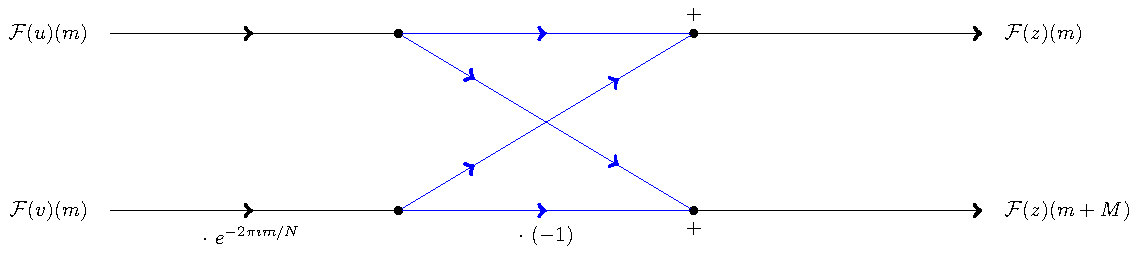
\includegraphics[width=1\textwidth]{./slike-latex/metulj}
\end{figure}
%

Kar smo pri postopku naredili je bilo to, da smo originalni problem izračuna Fourierove transformacije na vektorju dolžine $N$ z nekaj računske manipulacije prevedli na podproblema velikosti $N/2$. v primeru, ko bi bila vektorja iz podproblema ponovno sode velikosti, bi postopek lahko ponovili. Najbolj zaželjen primer za izračun DFT je zato v primeru, ko je $N$ potenca števila 2, tj.\ $N = 2^n$ za $n \in \N$. Za lažji zapis bomo uvedli oznako $E(n)$, s katero bomo označili zgornjo mejo potrebnmih kompleksnih množenj za izračun DFT vektorja dolžine $N$.
%
\begin{lema}
Naj bo $N = 2^n$ za $n \in \N$. Tedaj velja
\begin{equation*}
  E(N) \leq \frac{1}{2} N \log_2N \;.
\end{equation*}
\end{lema}
%
\begin{dokaz}
Dokaz naredimo z indukcijo na naravno število $n$. Baza indukcije je v primeru $n = 1$, ko je vektor $z$ dolžine 2, $z = (a, b)$. Z uporabo \eqref{} % deficiije, ko pomnožimo z matriko W
izračunamo $\F(z) = (a + b, a - b)$, za kar ne potrebujemo kompleksnih množenj. Dobimo, da je $E(2) \leq \frac{1}{2} 2 \log_2 2 = 1$, kar pomeni, da v primeru $n = 1$ lema velja. Predpostavimo sedaj, da lema velja za $n - 1$ in dokažimo, da velja za $n$. Iz postopka v prejšnji lemi je razvidno, da je za izračun vektorja $z$ dolžine $N = 2M$ potrebnih največ $2E(M) + M$ kompleksnih množenj. Z uporabo te opazke in indukcijske predpostavke sledi izračun
\begin{equation*}
  E(2^n) \leq 2 E(2^{n-1}) + 2^{n-1} \leq 2\frac{1}{2} 2^{n-1} \log_{2} 2^{k-1} + 2^{k-1} = k 2^{k-1} = \frac{1}{2} k 2^k = \frac{1}{2} N \log_2N \;,
\end{equation*}
ki pokaže, da lema velja za vsak $n \in \N$.
\end{dokaz}
%
Sedaj si bomo pogledali kako lahko hitro Fourierovo transformacijo uporabimo v primeru, ko $N$ ni sodo število. V primeru, ko je $N$ sestavljeno število, $N = pq$, lahko naredimo posplošitev zgornje leme.
%
\begin{lema}
Naj bosta $p, q \in \N$, $N = pq$ in $z \in \l^2(\Z_N)$. Za $k \in \set{0, 1, \ldots, q-1}$ definiramo zaporedje vektorjev $w_0, w_1, \ldots, w_{p-1} \in \l^2(\Z_q)$ s formulo
$$w_l(k) = z(kp + l).$$
Zaporedje vektorjev $v_0, v_1, \ldots, v_{q-1} \in \l^2(\Z_p)$ definiramo za $\l \in \set{0, 1, \ldots, p-1}$ s formulo
$$v_b(l) = e^{-\frac{2\pi\imath bl}{N}} \F(w)(b).$$
Tedaj za $a \in \set{0, 1, \ldots, p-1}$ in $b \in \set{0, 1, \ldots, q-1}$ velja
\begin{equation}\label{eq:aqb}
\F(z)(aq + b) = \F(v_b)(a).
\end{equation}
\end{lema}
%
\begin{dokaz}
%
Osnovni izrek o deljenju naravnih števil nam pove, da lahko vsako število $m \in \set{0, 1, \ldots, N-1}$ zapišemo v obliki $m = aq + b$ za $a \in \set{0, 1, \ldots, p-1}$ in $b \in \set{0, 1, \ldots, q-1}$. Torej znamo po lemi s formulo \eqref{eq:aqb} izračunati $\F(z)(m)$ za vsak $m \in \set{0, 1, \ldots, q-1}$.

Po osnovnem izreku o deljenju lahko zapišemo vsak $n \in \set{0, 1, \ldots, N-1}$ kot $n = kp + l$ za $k \in \set{0, 1, \ldots, p-1}$ in $l \in \set{0, 1, \ldots, q-1}$. Z uporabo tega zapisa števila $n$ in novo definiranimi zaporedji iz predpostavk leme izračunamo:
\begin{align*}
  \F(z)(aq + b) & = \sum_{n=0}^{N-1} z(n) e^{-\frac{2\pi\imath(aq + b)n}{N}} = \sum_{l=0}^{p-1} \sum_{k=0}^{q-1} z(kp + l)e^{-\frac{2\pi\imath(aq + b)(kp + l)}{pq}} \\
  & = \sum_{l=0}^{p-1} e^{-2\pi\imath al}{p} e^{-\frac{2\pi\imath bl}{N}} \sum_{k=0}^{q-1} w_l(k) e^{-\frac{2\pi\imath bk}{q}} = \sum_{l=0}^{p-1} e^{-\frac{2\pi\imath al}{p} e^{-\frac{2\pi\imath bl}{N}}} \F(w_l)(b) \\
  & = \sum_{l=0}^{p-1} e^{-\frac{2\pi\imath al}{p}} v_b(l) = \F(v_b)(a).
\end{align*}
\end{dokaz}
%
Sedaj pa si poglejmo kolikšno število kompleksnih množenj je potrebno v tem primeru. Po postopku, ki je nakazan v lemi, moramo najprej izračunati vektorje $\F(w_l)$ za $l \in \set{0, 1, \ldots, p-1}$. Za vsak posamezen $\F(w_l)$ potrebujemo $E(q)$ kompleksnih množenj, skupno torej $p E(q)$. Dobljene vektorje $\F(w_l)(b)$ dolžine $q$ moramo nato pomnožiti z $e^{-\frac{2\pi\imath bl}{N}}$, kar zahteva dodatnih $pq$ kompleksnih množenj. Ko tako dobimo vektorje $v_b(a)$, moramo izračunati $\F(v_b)(a)$ za $b \in \set{0, 1, \ldots, q-1}$, kar zahteva dodatnih $qE(p)$ kompleksnih množenj. Skupno je torej za izračun FFT vektorja dolžine $pq$ potrebnih
\begin{equation}
  E(pq) \leq pE(q) + qE(p) + pq
\end{equation}
kompleksnih množenj.

Kaj pa se zgodi v primeru, ko je $N$ praštevilo. Tedaj na vektorju ne moremo uporabiti FFT. vendar pa še ni vse izgubljeno, vektor lahko namreč na koncu podaljšamo z ničlami do željene velikosti, ki omogoča izvedbo FFT. Zaradi dodanih ničel namreč ne povzročimo velike škode, izračun pa postane opazno hitrejši.

Od tu dalje bomo sedaj predpostavili, da je $N$ potenca števila 2, tj.\ $N = 2^n$. Tedaj lahko $m \in \set{0,1 \ldots N-1}$ zapišemo v obliki polinoma $m = m_0 + m_1 2 + m_2 2^2 + \ldots + m_{n-1} 2^{n-1}$, kjer so $m_0, m_1, \ldots, m_{n-1} \in \set{0, 1}$. Za $z \in \l^2(\Z_N)$ bomo pisali $z(m) = z(m_{n-1}, m_n, \ldots, m_1, m_0)$. Za $k = k_0 + k_1 2 + k_2 2^2 + \ldots + k_{n-1} 2^{n-1}$, $k_0, k_1, \ldots, k_{n-1} \in \set{0, 1}$ izračunamo
%
\begin{align*}
  \F(z)(k) & = \sum_{m=0}^{N-1} z(m) e^{-\frac{2\pi\imath km}{N}} \\
  & = \sum_{m_0 = 0}^1 \sum_{m_1 = 0}^1 \cdots \sum_{m_{n-1} = 0}^1 z(m_{n-1}, m_{n-2}, \ldots, m_1, m_0) \cdot \\
 \cdot & exp\left(\frac{-2\pi\imath(k_0 + k_1 2 + k_2 2^2 + \ldots + k_{n-1} 2^{n-1})(m_0 + m_1 2 + m_2 2^2 + \ldots + m_{n-1} 2^{n-1})}{2^n}\right). 
\end{align*}
%
Eksponent razbijemo na produkte glede na vsoto $m_0 + m_1 2 + m_2 2^2 + \ldots + m_{n-1} 2^{n-1}$, poenostavimo dobljeni izraz in ga vstavimo v formulo za $\F(z)(k)$. Dobimo:
%
\begin{align*}
\F(z)(k) & = \sum_{m_0 = 0}^1 \sum_{m_1 = 0}^1 \cdots \sum_{m_{n-1} = 0}^1 z(m_{n-1}, m_{n-2}, \ldots, m_1, m_0) \cdot exp\left(\frac{-2\pi\imath k_02^{n-1}m_{n-1}}{2^n}\right) \\
&  \cdot exp\left(\frac{-2\pi\imath (k_0 + k_1 2)2^{n-2}m_{n-2}}{2^n}\right) \cdots exp\left(\frac{-2\pi\imath (k_0 + k_1 2 + \cdots +  k_{n-1} 2^{n-1}) m_0}{2^n}\right).
\end{align*}
%
Notranja vsota je odvisna od spremenljivk $m_0, m_1, \ldots, m_{n-2}$ in $k_0$, nič pa od $k_1, k_2, \ldots, k_{n-1}$. Lahko definiramo
\begin{align*}
  & y_1(k_0, m_{n-2}, m_{n-3},  \ldots, m_0)\\
  & = \sum_{m_{n-1}=0}^{1} z(m_{n-1},m_{n-2},\ldots,m_1,m_0) \cdot \exp\left(-\frac{2\pi\imath k_0 2^{n-1}m_{n-1}}{2^n}\right)\\
  & = z(0,m_{n-2},\ldots,m_1,m_0) \cdot 1 + z(1,m_{n-2},\ldots,m_1,m_0)\cdot \exp\left(-\frac{2\pi\imath k_0 2^{n-1}}{2^n}\right) \;.
\end{align*}
%
Izračun $y_1$ zahteva le eno kompleksno množenje za vsako izmed $2^n$ možnih vrednosti parametrov $k_0, m_{n-2}, m_{n-1}, \ldots, m_1, m_0$. Za izračun vseh možnih vrednosti izraza $y_1$ potrebujemo torej $2^n$ kompleksnih množenj.

Na naslednjem koraku lahko sedaj izračunamo $y_2$ s formulo
\begin{align*}
  & y_2(k_0, k_1, m_{n-3},  \ldots, m_0)\\
  & = \sum_{m_{n-1}=0}^{1} y_1(k_0, m_{n-2},\ldots,m_1,m_0) \cdot \exp\left(-\frac{2\pi\imath (k_0 + k_1 2) 2^{n-2}m_{n-2}}{2^n}\right) \;.
\end{align*}
%
Ta izračun prav tako potrebuje $2^n$ kompleksnih množenj. Naprej nadaljujemo podobno. Poglejmo si shemo, ki prikazuje kako izračunamo $z$:
%
\begin{align*}
 z(m_{n-1}, m_{n-2}, \ldots, m_1, m_0) & \to y_1(k_0, m_{n-2}, \ldots, m_1, m_0) \\
 y_1(k_0, m_{n-2}, m_{n-3},\ldots, m_0) & \to y_2(k_0, k_1, m_{n-3}, \ldots, m_0) \\
 & \vdots \\
 y_{n-1}(k_0, k_1, k_2, \ldots, k_{n-2}, m_0) & \to y_n(k_0, k_1, k_2, \ldots, k_{n-2}, k_{n-1}) \;.
\end{align*}
%
Kot smo rekli, na vsakem koraku potrebujemo $2^n$ kompleksnih množenj, imamo $n$ korakov, skupno torej $n\cdot 2^n = N \log_2N$ kompleksnih množenj. Poleg tega opazimo tudi, da po izračunu $y_{j}$ vektorja $y_{j-1}$ ne potrebujemo več. IZračune vektorje lahko torej delamo na mestu, kar pomeni, da lahko na vsakem koraku prejšnje podatke zamenjamo z novimi trenutnimi podatki.

Prav tako lahko z $\frac{N}{2} \log_2N$ kompleksnimi množenji izračunamo IDFT po formuli $\F^{-1}(w)(n) = \frac{1}{N} \F(w)(N-n)$.

S pomočjo DFT in IDFT lahko sedaj pospešimo tudi računanje konvolucije. Vemo namreč, da velja:
$$z \ast w = \F^{-1}(\F(z)\F(w)).$$
Skupno porabimo za izračun konvolucije $N + \frac{3N}{2}\log_2N$ kompleksnih množenj.
%
\subsubsection{Dvodimenzionalna hitra diskretna Fourierova transformacija}
Direkten izračun vseh vrednosti $y(n_1, m_2)$ zahteva $N_1 N_2^2$ kompleksnih množenj, za tem pa direkten izračun vseh vrednosti za $\hat{z}(m_1, m_2)$ zahteva $N_1^2 N_2$ kompleksnih množenj. Skupaj torej potrebujemo $N_1 N_2 (N_1 + N_2)$ množenj.
%
\begin{opomba}
Razlog za to izboljšavo računske zahtevnosti je ta, da 2D DFT sestoji, po definiciji, iz izračuna ene transformacije veliksoti $N_2$ (notranja vsota), ki ji sledi izračun transformacije velikosti $N_1$.  Izračunu, ki ga lahko razbijemo na zaporedje manjših vsot na ta način, pravimo \emph{paraleliziran}. To, da je FFT paraleliziran izračun sledi iz dejstva, da je DFT paraleliziran izračun.
\end{opomba}
%
\begin{trditev}
Naj bosta $N_1$ in $N_2$ števili potence 2. Z uporabo računanja od zgoraj namesto direktnega računanja, se da $\F(z)$ izračunati z uporabo največ $\frac{1}{2} N_1 N_2 \log_2(N_1 N_2)$ kompleksnih množenj.  
\end{trditev}
%
%%
%% Signal
\section{Transformacije slik}\label{sec:TransformacijeSlik}
%
%TODO Poveš kako bo predstavljena naša slika.
\subsection{Signali}\label{sec:Signali}
%
\emph{Signali} so funkcije ene ali več spremenljivk, ki nam posredujejo določene informacije o nekem fizikalnem pojavu, npr.\ podatke o zvočni frekvenci glasbila. Podatke, ki bi jih želeli dobiti iz vhodnega signala, največkrat ne dobimo direktno, temveč moramo vhodni signal pred njegovo analizo pretvoriti v nek drug sistem oz.\ zapis. Matematično povedano, na funkciji (matematični predstavitvi signala) moramo izvesti neko transformacijo. Predstavitev signala s funkcijo in transformacije, ki jih izvedemo na tej funkciji, so odvisne od lastnosti, ki jim preučevani signal ustreza (periodičnost, končnost, zveznost \ldots).
%
% TODO iz [0, 255], ker je digitalna slika
Slika je signal, ki ga uvrščamo v skupini diskretnih in digitalnih signalov. Če imamo sivinsko sliko, potem je osnovna predstavitev signala $n \times m$ matrika, ki ima vrednosti elementov z intervala $[0, 1]$. Pri tem sta $n$ višina in $m$ širina slike, vrednosti elementov pa nastavimo na vrednosti pripadajočih slikovnih točk. Sliko bomo označili z $I$, njene slikovne točke pa z $I(x, y)$.

\emph{Transformacijo slike} $I$ bomo označili s $T$ in jo definirali kot:
%
$$T: I(x, y) \to J(u, v).$$
%
Obravnavali bomo tri skupine transformacij:
%
\begin{enumerate}
\item točkovne transformacije (izhodna vrednost transformacije je odvisna le od ene vrednosti; ni nujno, da uporabimo pri izračunu vrednosti; 
\item lokalne transformacije (izhodna vrednost transformacije $T$ je odvisna od vseh vrednosti v soseski pripadajoče slikovne točke vhodne slike);
\item globalne transformacije (izhodna vrednost transformacije $T$ v točki $(x, y)$ je odvisna od vseh vrednosti vhodne slike).
\end{enumerate}
%
V nadaljevanju bomo spoznali posamezne skupine teh transformacij in njihovo praktično vrednost.
%
\subsection{Točkovne transformacije}
%
Točkovne transformacije pri izračunu vrednosti $T(x, y)$ uporabijo le podatek o vrednosti slikovne točke $(x, y)$ (glej sliko \ref{fig:tockovnaT}). Za izračun točkovne transformacije $T$ na $n \times m$ veliki sliki $I$ porabimo $\O(k\cdot nm)$ časa, pri čemer je $O(k)$ časovna zahtevnost izračuna vrednosti $T(x, y)$ za eno slikovno točko. Ker za izračun potrebujemo le vrednost dotične slikovne točke, lahko izvedemo računanje na mestu, torej pri računanju ne potrebujemo dodatnega pomnilnika.

%
\begin{figure}[htbp]
  \centering
  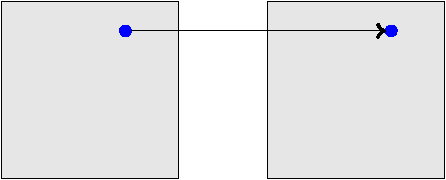
\includegraphics[width=0.6\textwidth]{./slike-latex/tockovnaT}
  \caption{Točkovna transformacija vhodne slike.}
  \label{fig:tockovnaT}
\end{figure}
%

Enostavni primeri točkovnih transformacij so: rotacija slike, zrcaljenje, skrčitev, \ldots % TODO une weird k swirl itd. dodaj
Za nas pomembne točkovne transformacije so tiste, ki spreminjajo barve itd. %TODO lepo napiši to
%% Lokalne transformacije
\subsection{Lokalne transformacije}\label{sec:LokalneTransformacije}
%
Pri lokalnih transformacijah za izračun $T(x, y)$ v slikovni točki $(x, y)$ uporabimo vrednosti slikovnih točk v njeni soseki (glej sliko \ref{fig:lokalnaT}).

%
\begin{figure}[htbp]
  \centering
  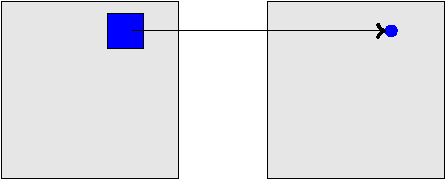
\includegraphics[width=0.6\textwidth]{./slike-latex/lokalnaT}
  \caption{Lokalna transformacija na sliki.}
  \label{fig:lokalnaT}
\end{figure}
%

Na področju obdelave slik so tovrstne transformacije uveljavljen postopek, ki mu pravimo \emph{filtriranje}. V tem kontekstu je $T(x, y)$ utežena vsota vrednosti slikovnih točk iz pravokotne okolice slikovne točke $(x, y)$. Uteži shranimo v \emph{filtrirno masko} $h$, ki je $(2b + 1)\times(2a + 1)$ matrika z realnimi vrednostmi. Običajno so filtrirne maske kvadratne in manjših velikosti. Vrednosti $T(x, y)$, ki jih dobimo pri filtriranju slike $I$ s filtrom $h$, izračunamo s pomočjo konvolucije:
%
\begin{equation}\label{eq:filtriranje}
T(x, y) = \frac{(I \ast h)(x,y)}{\sum_{s=-a}^{a} \sum_{t=-b}^{b} h(s, t)} = \frac{\sum_{s=-a}^{a} \sum_{t=-b}^{b} h(s, t) I(x-s, y-t)}{\sum_{s=-a}^{a} \sum_{t=-b}^{b} h(s, t)} \;.
\end{equation}
%
\begin{opomba}
V literaturi velikokrat poudarijo, da gre za filtriranje v slikovni domeni, saj poznamo tudi filtriranje v Fourierovi domeni, ki pa ga bomo mi spoznali malce kasneje.
\end{opomba}
%
\begin{opomba}
Kot vidimo v enačbi \eqref{eq:filtriranje}, smo rezultat, ki ga dobimo pri konvoluciji slike in filtrirne maske, normirali. Namesto tega bi lahko za filtrirno masko zahtevali, da je normirana (tj.\ ima vsoto vrednosti 1). Filtrirne maske, ki jih bomo predstavili v našem delu, bomo zapisali v normirani obliki. 
\end{opomba}
%
Postopek filtriranja obsega večji del področja pri obdelavi slik. Z uporabo filtrirnih mask lahko poiščemo, zgladimo ali izostrimo robove na sliki, zameglimo celotno sliko \ldots V nadaljevanju bomo predstavili primere filtrirnih mask, ki jih bomo kasneje tudi uporabljali v algoritmih za likovno upodabljanje slik.
%%% Tehnični pogled na filtriranje
\subsubsection{Tehnični pogled na filtriranje}\label{sec:TehnicniPogledNaFiltriranje}
%
Za boljšo predstavo bomo sedaj filtriranje predstavili še grafično. Filtrirno masko $h$ (glej \ref{fig:maskah}) najprej rotiramo za $180 \degree$, da dobimo filtrrino masko $h'$. Slednjo nato postavimo na vhodno sliko $I$ tako, da center maske sovpada s slikovno točko na sliki $I$, v kateri želimo izračunati vrednost $T(x, y)$. Vrednost $T(x, y)$ sedaj izračunamo tako, da pomnožimo istoležne vrednosti v matriki $h'$ in na sliki $I$ (glej sliko \ref{fig:pomnoziI}). Za razliko od točkovne transformacije, pri kateri smo novo vrednost lahko kar shranili na mesto $(x, y)$ v matriki $I$, moramo naračunane vrednosti shraniti v novo matriko $J$.

V primeru, ko želimo izračunati npr.\ vrednost $T(x, y)$ za slikovno točko v kotu slike, del filtrirne maske ne pokriva slike $I$. Da se izognemu temu problemu, sliko $I$, pred filtriranjem s filtrirno masko velikosti $(2a + 1) \times (2a + 1)$, obrobimo naokoli z $a$ celicami. Njihove vrednosti lahko nastavimo na več načinov (za primer glej sliko \ref{fig:obrobaI}). Pri tem opazimo, da lahko sedaj (ob privzetku, da filtrirane vrednosti računamo po vrsti) namesto, da za novo naračunane vrednosti ustvarimo novo matriko $J$, pri računanju vrednosti $T(x, y)$ novo vrednost shranimo na mesto $(x-a, y-1)$, saj te vrednosti ne bomo več potrebovali pri izračunu ostalih vrednosti. S tem v primeru velikih slik naredimo velik prihranek pri pomnilniku.
%
\begin{primer}
%TODO Zakaj ne poravna slikic ????

\begin{figure}[htbp]
  \centering%
  \begin{tabular}{cccc}
  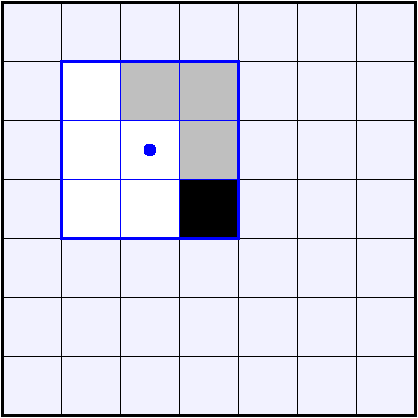
\includegraphics[width=0.2\textwidth]{./slike-latex/filter1}&
  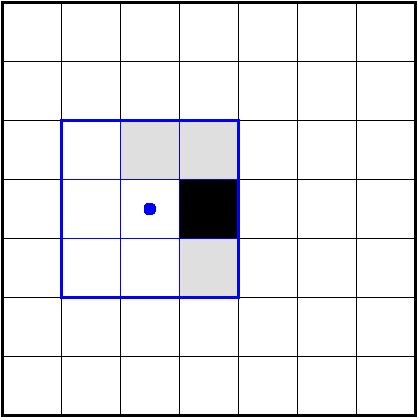
\includegraphics[width=0.2\textwidth]{./slike-latex/filter2}&
  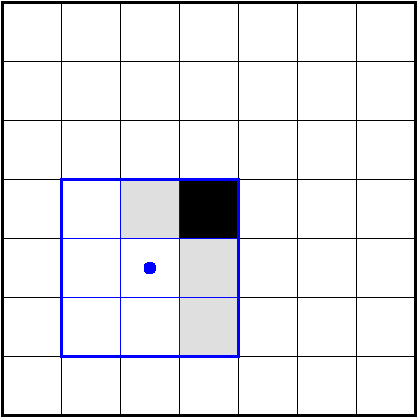
\includegraphics[width=0.2\textwidth]{./slike-latex/filter3}&
  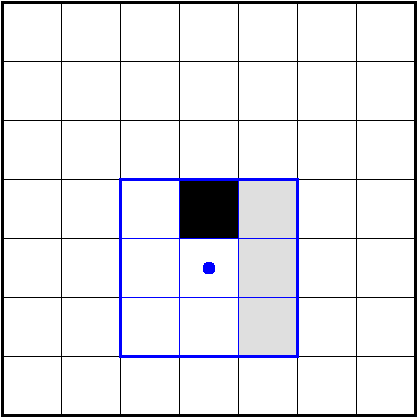
\includegraphics[width=0.2\textwidth]{./slike-latex/filter4}\\[0.4cm]
  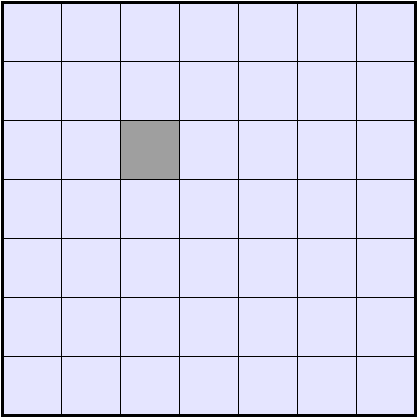
\includegraphics[width=0.2\textwidth]{./slike-latex/filter1s}&
  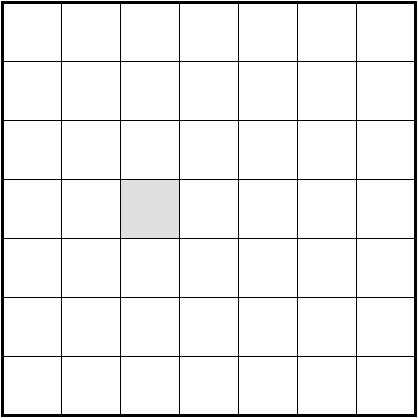
\includegraphics[width=0.2\textwidth]{./slike-latex/filter2s}&
  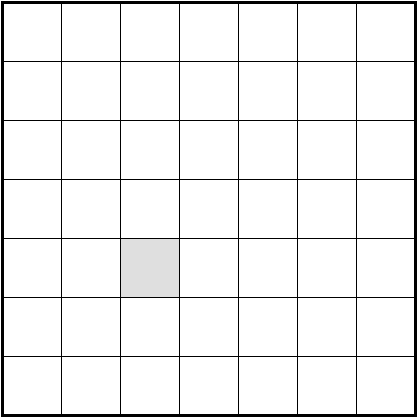
\includegraphics[width=0.2\textwidth]{./slike-latex/filter3s}&
  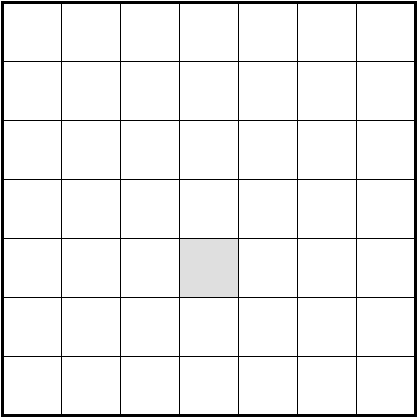
\includegraphics[width=0.2\textwidth]{./slike-latex/filter4s}
  \end{tabular}
  \caption{Filtriranje v slikovni domeni.}
  \label{fig:filtriranje}
\end{figure}

\end{primer}
%
Omenimo naj še, da so filtrirne maske, za razliko od maske v zgornjem primeru, običajno simetrične. Pri računanju filtriranih vrednosti lahko zato preskočimo rotacijo filtrirne maske, saj dobimo nazaj isto filtrirno masko.

Zgoraj predstavljeni postopek je osnovni način filtriranja. V naslednjem podrazdelku, kjer bomo izpeljali filter za zameglitev slike, pa bomo spoznali še drug pristop k filtriranju.
%
\subsubsection{Zamegljenje slike}\label{sec:ZamegljenjeSlike}
%
\emph{Impulzna slika} $\Delta_{p,q}$ je slika, ki ima vrednosti vseh slikovnih točk, razen ene z vrednostjo 1, enake 0. Definirana je kot:
$$
\Delta_{p,q}(x - p, y - q)=
\begin{cases}
  1 & \mbox{če } (x, y) = (p,q), \\ 
  0 & \mbox{sicer}.
\end{cases}
$$
%
Konvolucijo slike $I$ z $w$ uteženo impulzno sliko $\Delta_{p,q}$ izračunamo kot:
\begin{equation*}
[I \ast w\Delta_{p,q}](x,y) = w \cdot I(x - p, y - q) \;.
\end{equation*}
%
Postopek za izračun filtrirane slike:
%
\begin{enumerate}
  \item Za vsako celico filtrirne maske $h$ naredimo eno prazno matriko velikosti $(h+2a)\times(w+2a)$.
  \item V vsako izmed teh praznih matrik kopiramo vhodno sliko $I$ tako, da
\end{enumerate}
%
Na sliki \ref{fig:premakniSlike}
%
\begin{primer}
%TODO Zakaj ne poravna slikic ????

\begin{figure}[htbp]
  \centering
  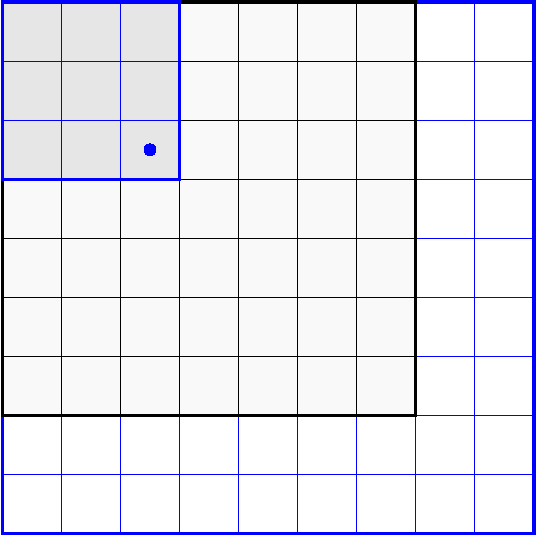
\includegraphics[width=0.2\textwidth]{./slike-latex/filterMSI1}\ \ \ \ \ \ 
  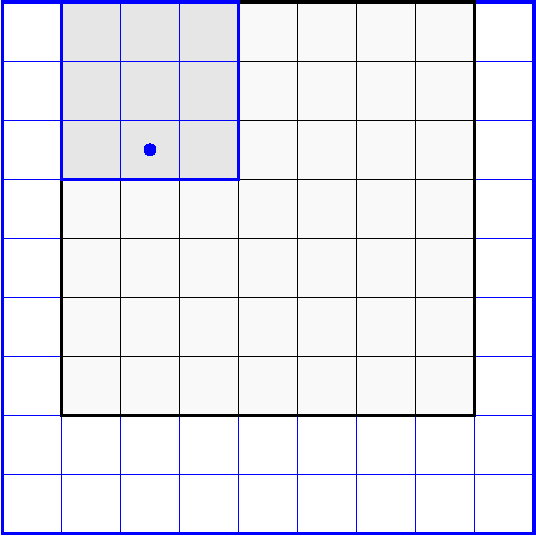
\includegraphics[width=0.2\textwidth]{./slike-latex/filterMSI2}\ \ \ \ \ \ 
  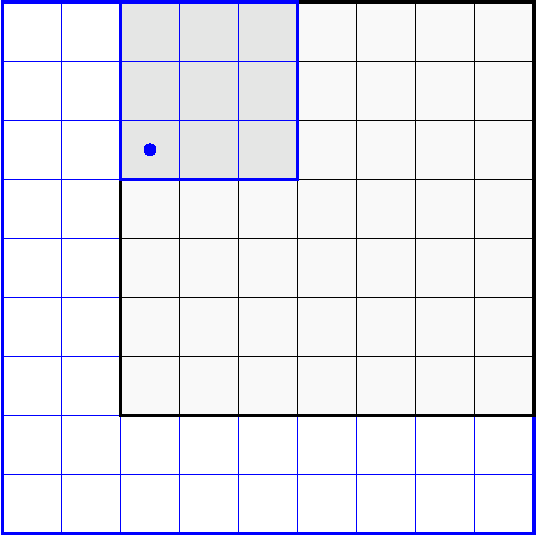
\includegraphics[width=0.2\textwidth]{./slike-latex/filterMSI3}\\[0.6cm]
  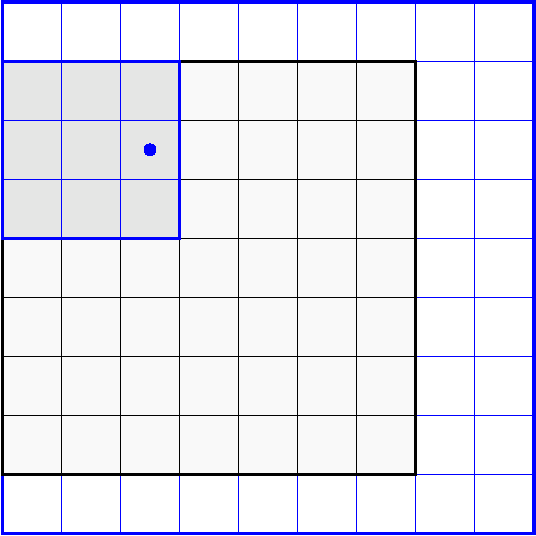
\includegraphics[width=0.2\textwidth]{./slike-latex/filterMSI4}\ \ \ \ \ \ 
  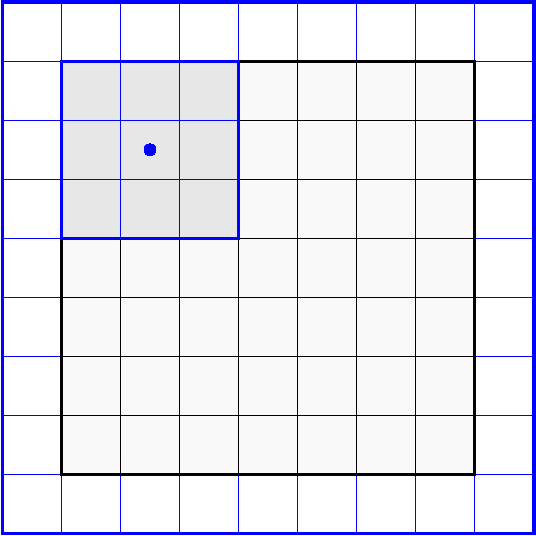
\includegraphics[width=0.2\textwidth]{./slike-latex/filterMSI5}\ \ \ \ \ \ 
  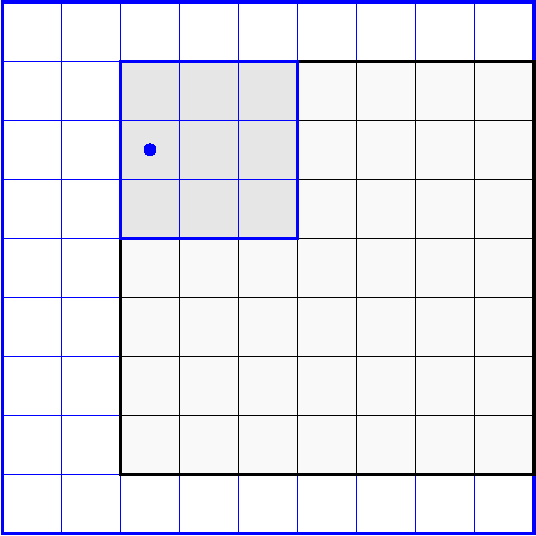
\includegraphics[width=0.2\textwidth]{./slike-latex/filterMSI6}\\[0.6cm]
  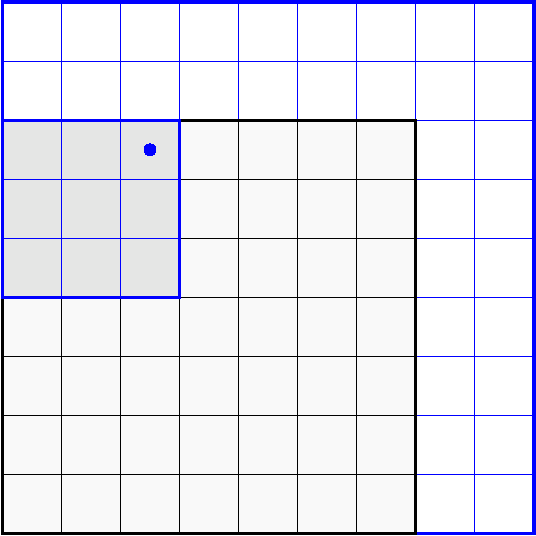
\includegraphics[width=0.2\textwidth]{./slike-latex/filterMSI7}\ \ \ \ \ \ 
  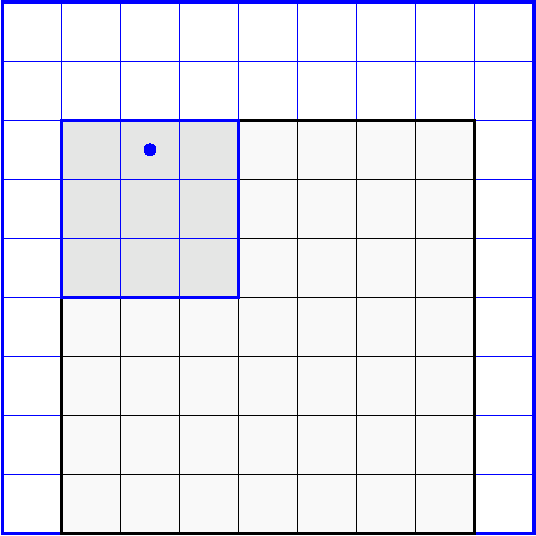
\includegraphics[width=0.2\textwidth]{./slike-latex/filterMSI8}\ \ \ \ \ \ 
  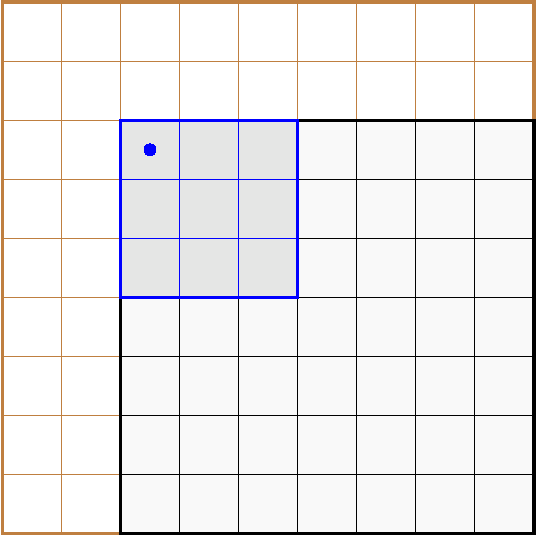
\includegraphics[width=0.2\textwidth]{./slike-latex/filterMSI9}
  \caption{Filtriranje v slikovni domeni.}
  \label{fig:filtriranje}
\end{figure}

\end{primer}
%
\subsubsection{Filter za zaznavo robov na sliki}
Kaj je rob ?

%
\begin{figure}[htbp]
  \centering
  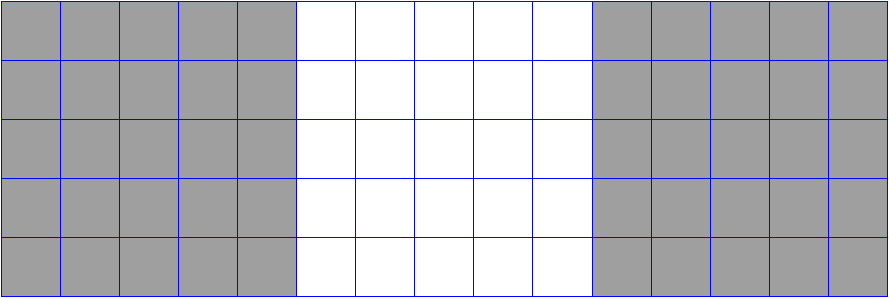
\includegraphics[width=0.45\textwidth]{./slike-latex/rob-slika}\ \ \ 
  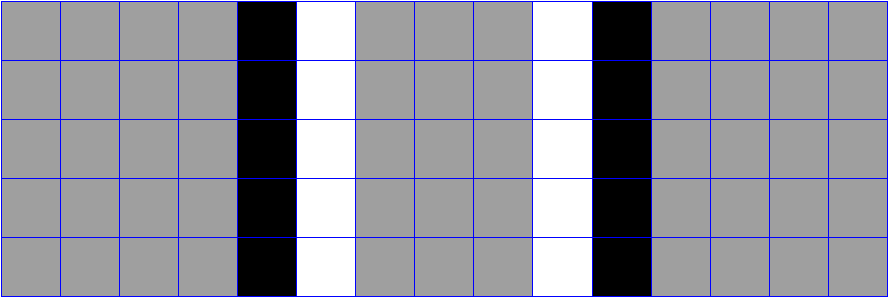
\includegraphics[width=0.45\textwidth]{./slike-latex/rob-center}\\[0.5cm]
  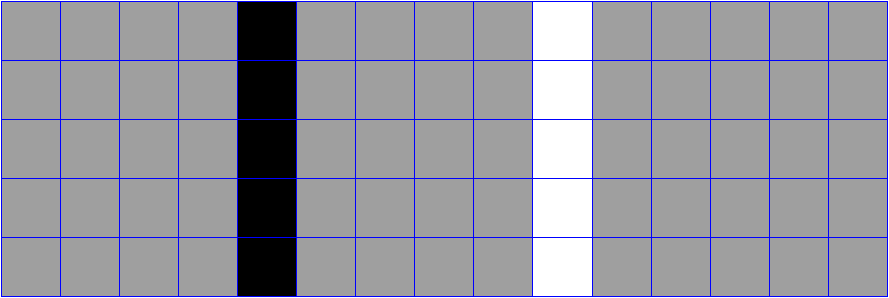
\includegraphics[width=0.45\textwidth]{./slike-latex/rob-naprej}\ \ \ 
  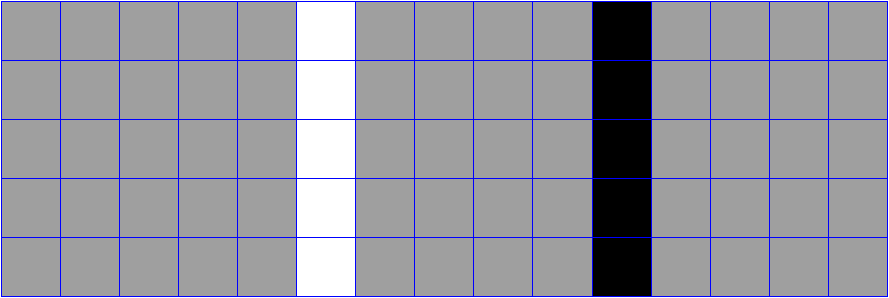
\includegraphics[width=0.45\textwidth]{./slike-latex/rob-nazaj}
  \caption{Robovi.}
  \label{fig:robovi}
\end{figure}
%

Ne maram ljudi.

%
\begin{figure}[htbp]
  \centering
  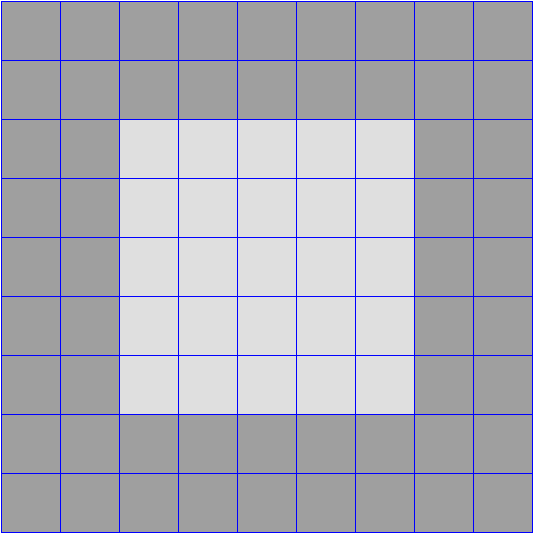
\includegraphics[width=0.23\textwidth]{./slike-latex/rob-kvadrat}\ \ \ 
  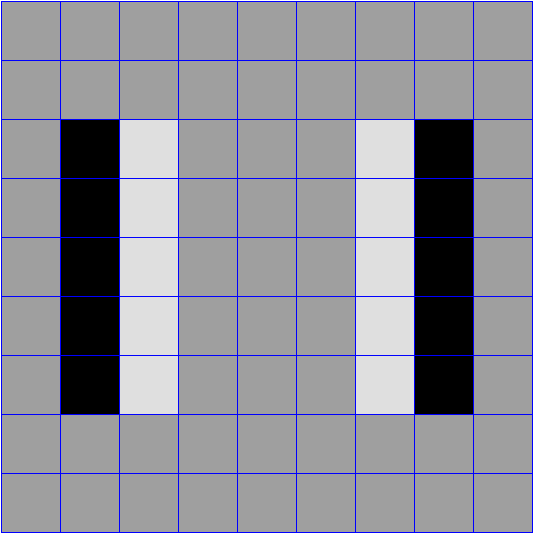
\includegraphics[width=0.23\textwidth]{./slike-latex/rob-kvadrat-vodoravno}\ \ \  
  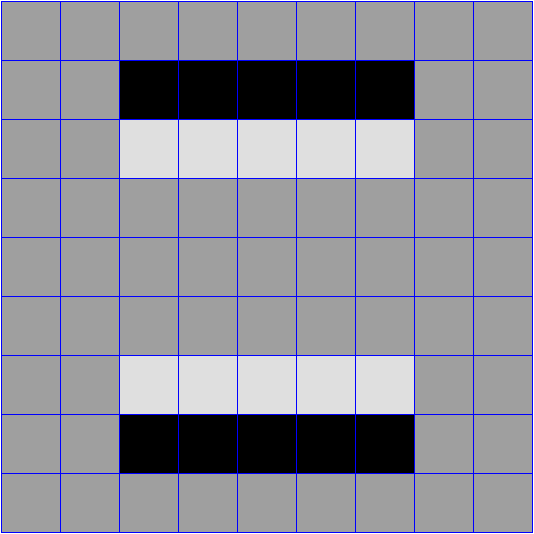
\includegraphics[width=0.23\textwidth]{./slike-latex/rob-kvadrat-navpicno}\ \ \ 
  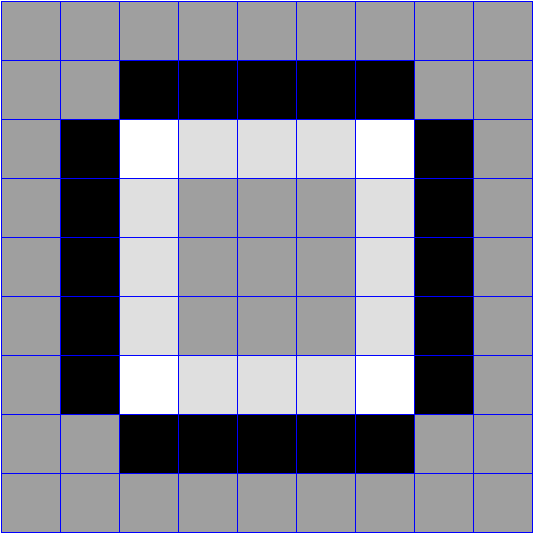
\includegraphics[width=0.23\textwidth]{./slike-latex/rob-kvadrat-vod-nav}
  \caption{Robovi v kvadratu.}
  \label{fig:roboviKvadrat}
\end{figure}
%
\subsection{Globalne transformacije}
Pri globalnih transformacijah za izračun vrednosti $T(x, y)$ upoštevamo vrednosti vseh slikovnih točk na sliki (glej sliko \ref{fig:globalnaT}). Najbolj pomembna transformacija te vrste je za nas Fourierova transformacija. V tem podrazdelku si bomo pogledali kakšna je praktična vrednost Fourierove transformacije pri obdelavi slik. 

%
\begin{figure}[htbp]
  \centering
  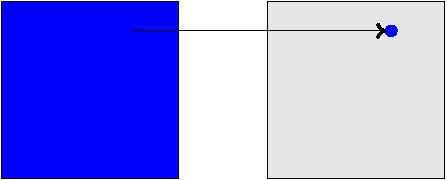
\includegraphics[width=0.6\textwidth]{./slike-latex/globalnaT}
  \caption{Globalna transformacija.}
  \label{fig:globalnaT}
\end{figure}
%

Kot smo videli v prvem razdelku tega poglavja lahko sliko $I$, namesto v običajni evklidski bazi, zapišemo v Fourierovi bazi:
%
\begin{equation*}
I(x, y) = \sum_{v = 0}^{N_1 - 1} \sum_{u = 0}^{N_2 - 1} \F(I)(u, v) F_{u, v}(x, y)\;.
\end{equation*}
%
Za vizualno predstavitev slike bomo na Fourierovo transformacijo pogledali z nekoliko bolj fizikalnega vidika. Za začetek si poglejmo dvodimenzionalne sinusoide.
%
\subsubsection{Dvodimenzionalne sinusoide}
 Zaradi poenostavitve zapisa naj velja $N_1 = N_2 = N$. Tedaj bomo zapisali $F_{u,v}(x,y)$ v polarni obliki:
%
$$F_{u, v}(x, y) = e^{\pm \imath \frac{2\pi \omega}{N}\cdot (u \sin \theta + v \cos \theta)},$$
%
kjer je $y = \omega \sin \theta$, $x = \omega \cos \theta$ in $\omega = \sqrt{x^2 + y^2}$.
%
Če pišemo še $\lambda = \frac{N}{\omega}$, dobimo
$$F_{u, v}(x, y) = \cos[\frac{2\pi}{\lambda} (u \sin \theta + v \cos \theta)] \pm \imath \sin[\frac{2\pi}{\lambda}(u \sin \theta + v \cos \theta)].$$
%
Tako realni del $F_{u, v}(x, y)$
$$\cos[\frac{2\pi}{\lambda} (u \sin \theta + v \cos \theta)]$$
kot imaginarni del
$$\pm \sin\left[\frac{2\pi}{\lambda}(u \sin \theta + v \cos \theta)\right]$$
sta sinusoidi z amplitudo $1$, periodo $\lambda$ in smerjo $\theta$.
%
Tedaj je $\frac{2\pi \omega}{N}$ radialna frekvenca, $\frac{\omega}{N}$ je frekvenca in $\lambda = \frac{N}{\omega}$ je dolžina vala sinusoide, merjena v slikovnih točkah.

Dvodimenzionalno sinusoido bomo zapisali s formulo
$$\frac{A}{2} \cdot \left(\cos\left[\frac{2\pi}{\lambda} \cdot (u \cdot \sin \Phi + v \cdot \cos \Phi) + \phi\right] + 1\right),$$
kjer je $A$ amplituda sinusoide in $\phi$ je fazni zamik.
%
\begin{definicija}
Naj bosta $Re$ in $Im$ realni in kompleksni del vrednosti $\F(I)(u, v)$. Definiramo pojme: 
%
\begin{enumerate}
\item \emph{Fourierov spekter}:
$$\abs{\F(I)(u, v)} = \sqrt{Re^2(u, v) + Im^2(u, v)};$$
\item \emph{fazni zamik}:
$$\varPhi(u, v) = \arctan\frac{Im(u, v)}{Re(u, v)};$$
\item \emph{močnostni spekter}:
$$P(u, v) = Re^2(u, v) + Im^2(u, v).$$
\end{enumerate}
\end{definicija}
%
Fourierovo transformacijo lahko z novo definiranimi pojmi zapišemo v polarni obliki:
$$\F(z)(u, v) = \abs{\F(z)(u, v)} e^{-\imath \cdot \varPhi(u, v)}.$$
%
Poveš, da če je pikica v frekvenčni domeni je to sinus v navadni evklidski ravnini.
%
\begin{primer}
Primer slike in njenega Fouirerovega spektra. In primer ene slike, ki bo neka vsota, nekaj nekaj baznih elemntov.
\end{primer}
%
\begin{primer}
Poglejmo si primer, ko imamo isti spekter in različni fazni zamik; ter isti fazni zamik, a različni spekter. Fazni zamik spreminjamo tako, da množimo z matriko $R$. Dobimo razne slike, ena izmed je lepa, ostale so kar nekaj ...             
\end{primer}
%
O spektru in faznem zamiku bomo govorili v nadaljevanju, saj sta to informaciji, ki nam povesta ogromno o sliki. Sedaj pa si najprej poglejmo še o translacijah in rotacijah Fourierove transformacije \ldots

%
\begin{figure}[htbp]
  \centering
  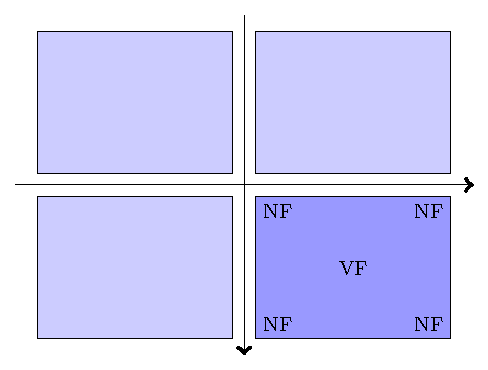
\includegraphics[width=0.49\textwidth]{./slike-latex/DFToriginal}
  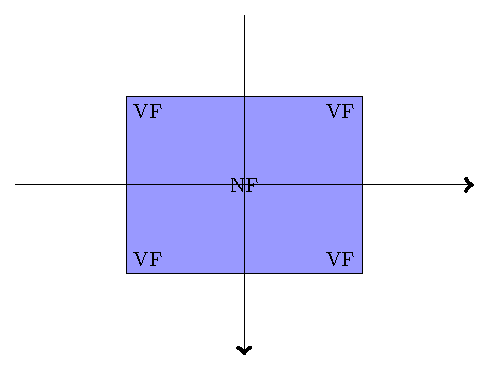
\includegraphics[width=0.49\textwidth]{./slike-latex/DFTpremaknjena}
  \caption{Originalna DFT.}
  \label{fig:DFToriginal}
\end{figure}
%
%%
\section{Barvni modeli}
Poznamo različne barvne modele:
%
\begin{itemize}
\item RGB barvni model;
\item CMY barvni model;
\item HSV barvni model;
\item HSL barvni model;
\item YUV barvni model.
\end{itemize}
%
\subsection{RGB in CMY barvna modela}
RGB barvni prostor predstavimo z enotsko kocko. Oglišča kocke so enaka:

\begin{figure}[htbp]
  \centering
  \subfigure[]{
  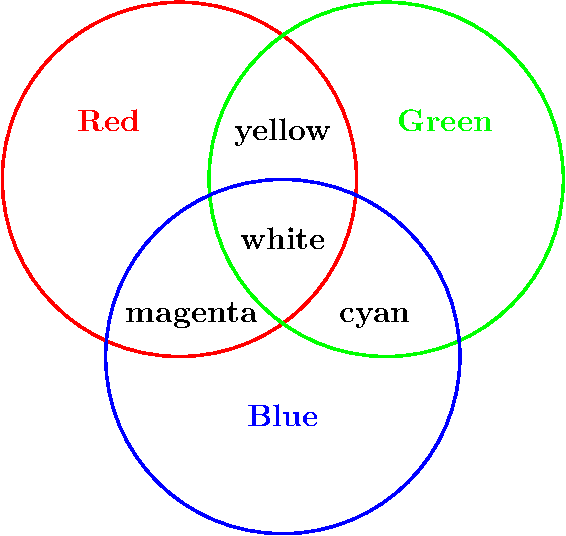
\includegraphics[width=0.31\textwidth]{./slike-latex/RGB}}
  \subfigure[]{
  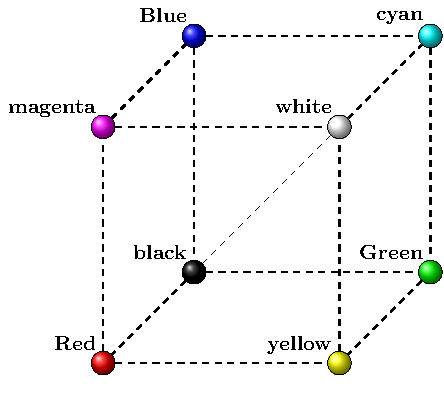
\includegraphics[width=0.31\textwidth]{./slike-latex/kockaRGB}}
  \subfigure[]{
  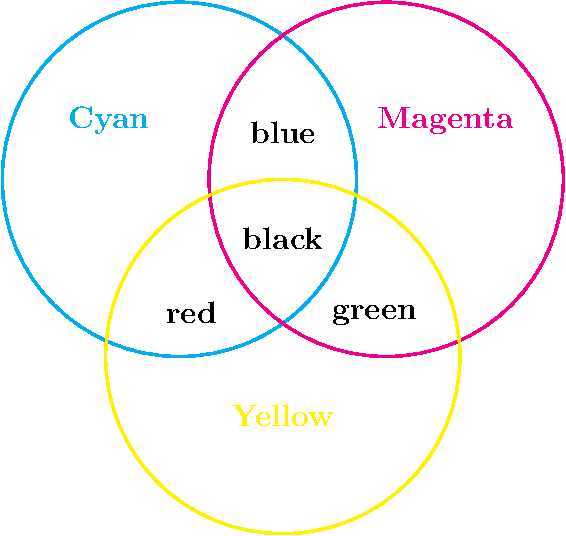
\includegraphics[width=0.31\textwidth]{./slike-latex/CMY}}
  \caption{RGB kocka.}
  \label{fig:rgbcube}
\end{figure}

%
\subsection{HSV in HSL barvna modela}
%
To je pa polarna predstavitev RGB barvnega modela.
%
\subsection{Kubelka--Monk barvni model}
%%
% Odstranjevanje šuma s slike.
\section{Odstranjevanje šuma na sliki}
%
Odstranjevanje (digitalnega) šuma predstavlja pomembno področje pri obdelavi slik, saj ta običajno povzroča motnje in nepravilnosti pri delovanju algoritmov, ki jih uporabljamo za obdelavo slik. Pri tem naj opozorimo, da s pojmom šum mnogi poimenujejo tudi fine strukture in teksture, ki so prisotne na sliki. Slednje namreč tudi predstavljajo težave, vendar pa se moramo njim izogniti pri samem algoritmu za obdelavo slik.

V tem razdelku bomo predstavili merilo uspešnosti za odpravljanje digitalnega šuma na sliki, ki je predstavljen v članku \cite{Buades:NLA}. Nadalje bomo primerjali različne metode, ki so predstavljene v tem članku, in nato metodo nelokalnega odstranjevanja šuma dopolnili z njeno pohitritvijo, opisano v članku \cite{Wang:fastNMD}. V zadnjem delu bomo nato predstavili še implementacije posameznih metod in primerjali eksperimentalno dobljene podatke o učinkovitosti posameznih metod.
%
\subsection{Metoda šuma}
Naj bo $I$ vhodna slika, na kateri je prisoten šum. Zaradi poenostavitve sintakse bomo slikovne točke, namesto z $(x, y)$, označili z $i = (x_i, y_i)$. Vrednosti slikovnih točk na sliki $I$ bomo označili z $v(i)$. Slednjo vrednost lahko zapišemo kot vsoto $v(i) = u(i) + n(i)$, pri čemer $u(i)$ predstavlja vrednost slikovne točke na sliki brez prisotnega šuma in $n(i)$ predstavlja vrednost prisotnega šuma. Z $v$ bomo označili množico vrednosti $v = \set{v(i) \mid i \in I}$, ki jo poimenujemo \emph{realna slika}. \emph{Originalna slika} je množica vrednosti $u = \set{u(i) \mid i \in I}$. Množica $n = \set{n(i) \mid i \in I}$ pa je pristoni \emph{šum} na sliki. Za modeliranje prisotnosti digitalnega šuma na sliki je najboljša izbira \emph{Gaussov beli šum}, tj.\ Gaussove vrednosti s srednjo vrednostjo 0 in standardnim odklonom $\sigma^2$.
%
\begin{definicija}
\emph{Operator šuma} $D_h$ je tak operator, za katerega lahko naredimo dekompozicijo realne slike $v$:
$$v = D_h v + n(D_h, v),$$
kjer je parameter $h$ odvisen od standardnega odklona šuma.
\end{definicija}
%
Od operatorja šuma pričakujemo, da bo množica (slika) $D_h v$ gladkejša od originalne slike. Za dobljeni šum $n(D_h v)$ pa želimo, da čimbolje aproksimira beli šum. Nočemo pa, da bi poleg digitalnega šuma na sliki operator šuma odstranil tudi morebitno prisotno teksturo in pokvaril videz drobnih detajlov na sliki. Ker večina metod deluje na principu povprečenja sosednjih vrednosti slikovnih točk, pa zgornje zahteve povečini pri metodah ne držijo v celoti. Za merilo uspešnosti posameznih metod oz.\ operatorja šuma bomo uvedli t.~i.\ \emph{metodo šuma}.
%
\begin{definicija}
Naj bo $u$ originalna slika in $D_h$ operator šuma, ki je odvisen od parametra $h$. \emph{Metoda šuma} je definirana kot razlika
$$u - D_h u.$$
\end{definicija}
%
Metoda šuma torej predstavlja razliko med originalno sliko $u$ (na kateri ni nujno prisoten šum) in $D_h u$ (originalna slika, na kateri smo uporabili operator šuma). V primeru, ko bi originalna slika vsebovala neko teksturo, vzorce ali določeno strukturo, se te v metodi šuma ne smejo pojaviti, saj bi to kazalo na to, da smo pokvarili videz originalne slike. Metoda šuma mora izgledati kot aproksimacija šuma, celo v primerih, ko je na originalni sliki šum prisoten v zelo majhnih količinah.
%%
\subsection{Lokalni algoritmi za odstranjevanje šuma na sliki}
Predstavili bomo tri metode za odstranjevanje šuma, ki pri računanju operatorja šuma izkoriščajo le lokalne podatke.
% 
% TODO kaj naredim, ker imam x pa y, rečem pa da imam slikovne točke i
\subsubsection{Gaussovo filtriranje}
Gaussovo filtriranje sodi v skupino izotropnega linearnega filtriranja slik, kjer naredimo konvolucijo slike z linearnim simetričnim filtrom. Gaussov filter definiramo s funkcijo
$$G_h(x) \coloneqq \frac{1}{4 \pi h^2} e^{- \frac{\abs{x}^2}{4 h^2}} \;.$$
V tem primeru ima $G_h$ standardni odklon $h$ in velja naslednji izrek.
%
\begin{izrek}
Metoda šuma za Gaussovo filtriranje je za dovolj majhen $h$ enaka
$$u - G_h \ast u = - h^2 \Delta u + o(h^2)\;.$$
\end{izrek}
%
Zgornji izrek dokažemo s pomočjo toplotne enačbe, saj izkoristimo dejstvo, da je fundamentalna rešitev toplotne enačbe porazdeljena po Gaussu (dokaz lahko bralec poišče v \cite{Lind:Gauss-dokaz}).

Izrek nam pove, da bo v harmoničnih delih slike metoda šuma enaka 0, medtem ko bo v bližini linij, robov in delov teksture imela visoke vrednosti. Na zveznih območjih slike bo metoda šuma torej optimalna, saj bo v celoti odstranila prisotni šum in pri tem ohranila videz slike. Deli slike v okolici linij, robov in prisotne teksture na sliki bodo po odstranitvi šuma postali zamegljeni in s tem pokvarili videz slike.
%%
\subsubsection{Anizotropno filtriranje}
Ideje za to vrsto filtriranja so bile predstavljene v \cite{Perona-Malik}. Pri anizotropnem filtriranju (kratica AF) poskušamo dejstvo, da pri Gaussovem filtriranju dobimo zamegljene dele slike, popraviti s tem, da v slikovni točki $i$ naredimo konvolucijo s filtrom $G_h$ le v smeri, ki je ortogonalna na $G(i)$. Pri tem je $G = \sqrt{(\partial_x u)^2 + (\partial_y u)^2}$, $\partial_x u$ in $\partial_y u$ sta gradientni sliki v $x$ in $y$ smeri. Konvolucijo naredimo torej le v ``smeri linije, ki poteka skozi slikovno točko~$i$.''

Operator šuma za AF je za $x$, $G(x) \neq 0$, definiran s funkcijo
%
$$AF_h u(x) = \int G_h(t)\cdot u\left( x + t \frac{G(x)^\perp}{\abs{G(x)}}\right) dt\;.$$
%
Ob predpostavki, da je originalna slika $u$ dvakrat zvezno odvedljiva v $x$, lahko s pomočjo Taylorjeve vrste drugega reda pokažemo veljavnost naslednjega izreka (dokaz bomo tukaj izpustili).
%
\begin{izrek}
Metoda šuma za anizotropni filter $AF$ je na območjih, kjer velja $Du(x) \neq 0$, enaka
$$u(x) - AF_h u(x) = - \frac{1}{2} h^2 \abs{G}\cdot \kappa (u)(x) + o(h^2)\;.$$
\end{izrek}
%
V metodi šuma se pojavi ukrivljenost krivulje $\kappa (u)(x)$, saj je uspešnost te metode odvisna od ukrivljenosti krivulje, ki poteka skozi točko. V bližini slikovnih točk, kjer je linija, ki poteka skozi, lokalno ravna, je metoda šuma enaka 0. Posledično se ravne linije in robovi pri tej vrsti filtriranja šuma zelo lepo ohranijo. V okolici slikovnih točk, kjer imajo linije veliko ukrivljenost in so vrednosti gradienta velike, pa metoda šuma doseže velike vrednosti. Posledično na zveznih delih slike in v okolici linij, ki imajo veliko ukrivljenost, dobimo zamegljeno sliko.
%%
\subsubsection{Sosedsko filtriranje}
\emph{Sosedsko filtriranje} je skupno ime za skupino filtriranj, pri katerih novo vrednost slikovne točke $i$ določimo na podlagi povprečja vrednosti tistih slikovnih točk iz njene soseske, ki imajo podobno vrednost. 

Leta 1985 je Yaroslavsky v \cite{Yaro:Digital} predstavil filter te vrste. Operator šuma je za $x \in \Omega$ definiral s funkcijo
%
$$YNF_{h, \rho} u(x) \coloneqq \frac{1}{C(x)} \int_{B_{\rho}(x)} u(y) e^{- \frac{\abs{u(y) - u(x)}^2}{h^2}} dy\;,$$
%
kjer je normalizacijska konstanta definirana kot $C(x) = \int_{B_{\rho}(x)} e^{-\frac{\abs{u(y) - u(x)}^2}{h^2}} dy$.
Za sosesko slikovne točke $x$ je izbral fiksno okolico $B_{\rho}(x)$, katere velikost je odvisna od parametra $\rho$. S filtrirnim parametrom $h$ pa nadzira katere vrednosti slikovnih točk bomo vzeli v povprečje. Ker pri računanju povprečja uporabimo le slikovne točke s podobno vrednostjo, se na ta način izognemu zamegljenju linij in robov.

Deset let kasneje je bil predstavljen bolj prepoznavni filter t.~i.\ SUSAN \cite{Susan:Filter}, pri katerem ne fiksiramo območja po katerem integriramo, temveč integrand pomnožimo z izrazom $e^{-\frac{\abs{y - x}^2}{\rho^2}}$. V tem izrazu, podobno kot pri YNF, s parametrom $\rho$ določimo soseko slikovnih točk, ki jih bomo upoštevali pri računanju povprečja. Operator šuma je definiran s funkcijo
%
$$SNF_{h, \rho} u(x) \coloneqq \frac{1}{C(x)} \int_{\Omega} u(y) e^{-\frac{\abs{y - x}^2}{\rho^2}} e^{- \frac{\abs{u(y) - u(x)}^2}{h^2}} dy\;,$$
%
kjer je normalizacijska konstanta definirana kot $C(x) = \int_{\Omega} e^{- \frac{\abs{y - x}^2}{\rho^2}} e^{- \frac{\abs{u(y) - u(x)}^2}{h^2}}$.

V praksi se operatorja šuma $YNF_{h, \rho}$ in $SNF_{h, \rho}$ obnašata podobno. Uporabljeni pristop za izbiro slikovnih točk, ki jih bomo upoštevali pri povprečju, v okolici linij in robov poskrbi, da pri računanju ne bomo hkrati vzeli v povprečje vrednosti, ki nastopijo na robu in v njegovi bližini. Na ta način se izognemu pojavu zamegljenosti robov po filtriranju. Vendar pa sosedski filter odpove v primeru, ko je v slikovnih točkah, ki jih primerjamo med seboj, prisoten šum. Tedaj namreč dobimo lažno območje slikovnih točk s podobno vrednostjo. Slednje vodi do umetnega pojava nepravilnosti na filtrirani sliki. Problem nastane zato, ker v integrandu primerjamo le vrednosti dveh slikovnih točk, nič pa ne upoštevamo geometrijske sestave njunih okolic. Na ta način ne zaznamo, da je v teh dveh slikovnih točkah prisoten šum, ki daje lažno prepričanje, da sta vrednosti podobni. Natančno opredeljen izrek, ki podpira trditve v tem odstavku, lahko bralec skupaj z dokazom najde v \cite[strani 10--13]{Buades:PDE}.
%%
\subsection{Nelokalni algoritem za odstranjevanje šuma na sliki}
Naj bo dana realna slika $v = \set{v(i) \mid i\in I}$. Za razliko od prejšnih metod, kjer smo vrednost za slikovno točko $i$ naračunali le na podlagi vrednosti, ki se nahajajo v njeni bližini, bomo sedaj pri računanju uporabili vrednosti vseh slikovnih točk. S tem bomo sicer zelo povečali računsko zahtevnost algoritma, vendar bomo slednjo nato v praksi zmanjšali s premišljeno uporabo nekaterih podatkovnih struktur in omejitvijo območja, ki ga bomo uporabili pri računanju vrednosti v slikovni točki $i$.
%
\subsubsection{Predstavitev postopka}
Najprej bomo definirali vrednost $NL(v)(i)$, ki jo izračunamo kot uteženo povprečje vseh slikovnih točk:
%
$$NL(v)(i) \coloneqq \sum_{j\in I} w(i, j) v(j)\;,$$
%
kjer je $\set{w(i, j)}_j$ množica uteži, ki zadošča pogojema $0 \leq w(i, j) \leq 1$ in $\sum_j w(i, j) = 1$.

Namesto, da bi primerjali le vrednosti slikovnih točk $i$ in $j$, bomo utež $w(i, j)$ definirali kot merilo podobnosti okolic slikovnih točk $i$ in $j$. Okolico slikovne točke $k$ označimo z $\NN_k$. Utež $w(i, j)$ bo odvisna od podobnosti vrednosti $v(\NN_i)$ in $v(\NN_j)$. Izračunali jo bomo z evklidsko razdaljo $\norm{v(\NN_i) - v(\NN_j)}_{2, a}^2$, kjer je $a > 0$ standardni odklon Gaussovega jedra. Uporabo evklidske razdalje za izračun podobnosti utemeljimo z izračunom matematičnega upanja razdalje $\norm{v(\NN_i) - v(\NN_j)}_{2, a}^2$, ki da rezultat
%
$$E[\norm{v(\NN_i) - v(\NN_j)}_{2, a}^2] = \norm{u(\NN_i) - u(\NN_j)}_{2, a}^2 + 2 \sigma^2.$$
%
Pri računanju podobnosti dveh območij s prisotnim šumom, bomo torej dobili enako stopnjo podobnosti, kot bi jo dobili v primeru, ko šum ni prisoten. S tem smo se izognili problemu, ki smo ga imeli pri sosedskem filtriranju.

Utež $w(i, j)$ izračunamo s formulo
%
$$w(i, j) = \frac{1}{Z(i)} e^{-\frac{\norm{v(\NN_i) - v(\NN_j)}_{2, a}^2}{h^2}},$$
%
kjer je normalizacijska konstanta $Z(i)$ enaka
%
$$Z(i) = \sum_j  e^{-\frac{\norm{v(\NN_i) - v(\NN_j)}_{2, a}^2}{h^2}}.$$
%
Utež $w(i, j)$ bo torej poskrbela, da bomo pri izračunu nove vrednosti za slikovno točko $i$, povprečili le vrednosti tistih slikovnih točk, ki imajo podobno geometrijsko strukturo v okolici.
%
\begin{primer}
\end{primer}
%
%TODO h nastavimo na 10 krat sigma
\subsubsection{Pravilnost postopka}
Če upoštevamo stacionarnost, potem algoritem NL-povprečenja konvergira k vrednosti pogojnega matematičnega upanja za piksel $i$. V tem primeru stacionarnost pomeni, da se z večanjem velikosti slike ohranijo podobna območja z detajli na sliki.

Naj bo $V$ naključno polje in $v$ njegova realizacija. Z $Z$ označimo zaporedje $Z_i = \set{X_i, Y_i}$, kjer je $Y_i = V(i)$ realna vrednost in je $X_i = V(\NN_i\backslash\set{i})$ vektor iz $\R ^p$. NL-povprečenje vzamemo kot pogoj pri pogojnemu matematičnemu upanju, izračun je tak
$$r(i) = E[Y_i \mid X_i = v(\NN_i\backslash\set{i})].$$

\begin{izrek}
Naj bo $Z = \set{V(i), V(\NN\backslash \set{i})}$ za $i = 1, 2 \ldots$ popolnoma stacionaren in mešan proces. Z $NL_n$ označimo algoritem NL-povprečenja, ki ga uporabimo na zaporedju $Z_n = \set{V(i), V(\NN_i \backslash \set{i})}_{i=1}^n$. Potem velja
$$\abs{N_n(j) - r(j)} \to 0$$
skoraj za vsak $j \in \set{1, \ldots, n}$.
\end{izrek}

Zgornji izrek nam pove, da algoritem NL-povprečenja popravi sliko s šumov in ne poskuša ločiti narazen šuma in originalne slike.

V tem primeru predpostavimo, da imamo aditiven bel šum. Naslednji rezultati nam povedo, da je pogojno matematično upanje funkcija $V(\NN_i\backslash \set{i})$, ki minimizira povprečno kvadratno napako za pravo sliko (originalno).

\begin{izrek}
Naj bodo $V, U$ in $N$ naključna polja, za katera velja, da je $V = U + N$, kjer je $N$ neodvisno od signala prisoten bel šum. Tedaj veljata naslednji trditvi:
\begin{enumerate}
\item Za vsak $i \in I$ in $x \in \R^p$ velja $E[V(i) \mid X_i = x] = E[U(i) \mid X_i = x]$.
\item matematično upanje $E[U(i) \mid V(\NN_i \backslash \set{i})]$ je funkcija v odvisnosti od $V(\NN_i \backslash \set{i})$, ki minimizira kvadrat napake
$$\min_g E[U(i) - g(V(\NN_i \backslash \set{i}))]^2.$$
\end{enumerate}
\end{izrek}
%
\subsubsection{Časovna zahtevnost}
Kljub temu, da nelokalni algoritem za odstranjevanje šuma, da zelo dobre rezultate in je robusten, pa je njegova uporaba zaradi visoke časovne zahtevnosti dokaj omejena.

Recimo, da je velikost slike $n^2$ in velikost okolice $\NN_k$ enaka $M^2$ ($M$ je konstanta). Časovna zahtevnost za izračun uteži $w(i, j)$ je enaka $M^2$. Izračun vrednosti $NL(v)(i)$ zahteva izračun $n^2$ uteži, kar pomeni, da je časovna zahtevnost izračuna ene vrednosti $NL(v)(i)$ enaka $\O(M^2\cdot n^2)$. Skupna časovna zahtevnost je torej $\O(M^2 \cdot n^4)$, saj moramo izračunati vrednost $NL(v)(i)$ za vsako izmed $n^2$ slikovnih točk.

Prva izboljšava, ki jo naredimo v praksi za zmanjšanje časovne zahtevnosti, je omejitev območja pri računanju vrednosti $NL(v)(i)$. Namesto, da vsoto naredimo po vseh slikovnih točkah, jo naredimo le na omejeni okolici slikovne točke $i$. V članku izbrana velikost je $21 \times 21$. Skupaj z izbiro $M = 7$ dobimo izboljšano časovno zahtevnost $\O(49\cdot 441\cdot n^2)$. Pridobili smo kvadratno časovno zahtevnost, kar pa še vedno ni dobro za širšo uporabo nelokalnega filtra v praksi. Poleg tega omejitev območja prinese slabšo kakovost filtrirane slike.
%
\subsubsection{Pohitritev algoritma}
Wang je skupaj s sodelavci v članku \cite{Wang:fastNMD} predstavil algoritem za nelokalno odstranjevanje šuma, ki v praksi porabi občutno manj časa za izračun kot originalni algoritem, pri čemer pa ohrani kakovost filtriranja. Kot smo videli, največ časa porabimo za izračun evklidske razdalje med dvema okolicama. Za to razdaljo bomo uvedli novo oznako $S(i, j)$:
%
\begin{align} \label{eq:zrcalna-slika}
  S(i, j) & = \norm{\NN_i - \NN_j}^2 \\
          & = \sum_{l=0}^{M-1} \sum_{m=0}^{M-1} [v(\NN_i)(l, m) - v(\NN_j)(l, m)]^2 \;.
\end{align}
%
Če sliko $I$ postavimo v koordinatni sistem in jo zrcalimo preko koordinatnega izhodišča (glej sliko \ref{fig:zrcalna-slika}), lahko $\NN_j(l, m)$ zapišemo kot $\NN_j(l - x_j', m - y_j')$, kjer je $x_j' = \frac{3M}{2} + x_j$ in $y_j' = \frac{3M}{2} + y_j$. Enačba \eqref{eq:zrcalna-slika} se s tem prepiše v obliko:
%
\begin{align*}
S(i, j) & = \sum_{l=0}^{M-1} \sum_{m=0}^{M-1} [v(\NN_i)(l, m) - v(\NN_j)(l - x_j', m - y_j')]^2 \\
         & = N_i^2 + N_j^2 - N_i \ast N_j \;,
\end{align*}
%
kjer so
%
\begin{align*}
N_i^2 & = \sum_{l=0}^{M-1} \sum_{m=0}^{M-1} (v(\NN_i)(l, m))^2, \\
N_j^2 & = \sum_{l=0}^{M-1} \sum_{m=0}^{M-1} (v(\NN_j)(l - x_j', m - y_j'))^2, \\
N_i \ast N_j & = 2 \cdot \sum_{l=0}^{M-1} \sum_{m=0}^{M-1} (v(\NN_i)(l, m) \cdot v(\NN_j)(l - x_j', m - y_j'))\;.
\end{align*}
%
Vrednosti $N_i^2$ in $N_j^2$ lahko s pomočjo podatkovne strukture \emph{vsote kvadratov} (\emph{angl.\ Summed Square Image}), ki je predstavljena v \ref{sec:vsota-kvadratov},  izračunamo brez uporabe množenj. 
%
\subsubsection{Vsota kvadratov}\label{sec:vsota-kvadratov}
Za slikovno točko $(x_0, y_0)$ naj bo
%
$$SSI[y_0, x_0] \coloneqq \sum_{x \leq x_0, y \leq y_0} v^2(y, x).$$

%
\begin{algorithm}
  \caption{Izračun $n \times m$ matrike vsote kvadratov.}
  \label{alg:SSI}
\begin{algorithmic}[1]
  \State $SSI$ $\leftarrow$ Prazna $n \times m$ matrika.
  \State $SSI[0,0]$ $\leftarrow$ $v^2(0,0)$
  \For {$x_0 \in \set{1, \ldots, m-1}$}
    \State $SSI[0, x_0]$ $\leftarrow$ $SSI[0, x_0 - 1] + v^2(0, x_0)$
  \EndFor
  \For {$y_0 \in \set{1, \ldots, n-1}$}
    \State $SSI[y_0, 0]$ $\leftarrow$ $SSI[y_0 - 1, 0] + v^2(y_0, 0)$
  \EndFor
  \For {$x_0 \in \set{1, \ldots, m-1}$}
    \For {$y_0 \in \set{1, \ldots, n-1}$}
      \State $SSI[y_0, x_0]$ $\leftarrow$ $SSI[x_0 - 1, y_0] + SSI[x_0, y_0 - 1] - SSI[x_0 - 1, y_0 - 1] + v^2(y_0, x_0)$
    \EndFor
  \EndFor
\end{algorithmic}
\end{algorithm}
%

Zgornji algoritem ima časovno zahtevnost $O(nm)$, pri čemer je $n \times m$ velikost slike. Vsako slikovno točko po zgornjem algoritmu namreč obiščemo natanko enkrat.

Če nas sedaj zanima kolikšna je vsota kvadratov vrednosti slikovnih točk na pravokotnem  imamo dano strukturo $SSI$, lahko vrednost poljubnega dela slike ali slikovne točke izračunamo v konstantnem času. Naj bo $D$ območje za katerega želimo izračunati vsoto kvadratov vrednosti. Vrednost $S_D$ določimo na naslednji način:
%
\begin{align*}
S_D & = S_{A \cup B \cup C \cup D} + S_A - S_{A \cup C} - S_{A \cup B} \\
       & = SSI(x_1, y_1) + SSI(x_0, y_0) - SSI(x_0, y_1) - SSI(x_1, y_0).
\end{align*}
%

%
\begin{figure}[htbp]
  \centering
  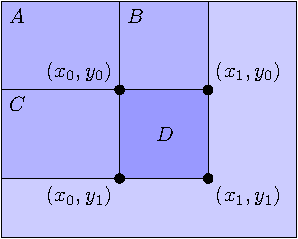
\includegraphics[width=0.3\textwidth]{./slike-latex/ssi}
\end{figure}
%
\subsection{Implementacija in primeri}